\section{Ocean tide prediction}
\label{sec:tidesOverview}
%-----------------%
\begin{quote}
Tidal prediction is the oldest form of ocean prediction, and is still the most accurate \citep{Parker:2007wq}. 
\end{quote}
%-----------------%
\subsection{Why it is worth unpacking ocean tides}
\label{sec:semantics}
The topic of ocean tides is particularly rich in ambiguous terminology and the potential for miscommunication is a real risk for operational forecasting.  The need to unpack some historical background and common definitions is unavailable. 

Tidal methods of analysing and forecasting the ocean have a long legacy in the history of western science.  Economically significant tidal sea level predictions in fact pre-date the whole modern scientific enterprise, and the evolution of the tidal perspective mirrors much of the story of classical continuum physics.

The \cite{Cartwright:2000tt} telling of the history of ocean tide science is illustrative. Remarkably, and perhaps typically, this scientific history of tides never even attempts to pin down a definition of what tide really should mean.  This surely deliberate exclusion stands in stark contrast to the minutiae of historical approaches and formulations and that the history covers.  The absence of definition may be read as an assertion that the \emph{history itself} is the only meaningful way to frame the scope of tidal science.
\cite{Pugh:1996uz} at least addresses the question of definition explicitly and in doing so casts a very wide net that catches almost anything that can be considered periodic.
\begin{quote}
Although any definition of tides will be somewhat arbitrary, it must emphasize this periodic and regular nature of the motion, whether that motion be of the sea surface level, currents, atmospheric pressure or earth movements. We define tides as periodic movements which are directly related in amplitude and phase to some periodic geophysical force \ldots.
\end{quote}
It is notable that whilst for Pugh \emph{periodicity} is a key feature of anything that is `tidal', he does not lock this periodicity to astronomy.  Pugh's pragmatic definition appears to be designed to best accommodate the conventional methods of harmonic analysis and sea level prediction that are so well established in operational agencies. Whilst this periodicity-stressing definition sensibly reflects the context of Pugh's text, it is certainly not the only working conceptualisation of what constitutes ocean tides; either within the operational forecasting context or in academic settings. 

In contrast to the periodic definition, most modern authors place the tidal potential in a defining role. Such an emphasis on the tidal potential or Astronomical Tide Generating Forces \ATGP{} reflects a greater regard for dynamics and inputs, as opposed to observed outputs, that is more complimentary to the wider field of geophysical fluid dynamics.  
\cite{Hendershott:1981ub} treats ocean tides as that subset of oceanographic long waves driven by the \ATGP{}.  Notably his discussion is careful with the distinction between dynamics and `practical tide prediction'. But even Henderscott's primarily dynamical perspective is imbued with the cultural interplay of physics and pragmatic prediction; as illustrated by his inclusion of the rather aphysical radiational potential concept associated with the \cite{Munk:1966ts} response method tradition.
The Australian Tide Manual \cite{PCTMSL-sp9} similarly reflects the historical intertwining of tidal physics and practical prediction methods; such that any forcing physics simply provides a backdrop to the singular focus on harmonic prediction.   
A step removed from ocean prediction, \cite{10.1016/b978-0-444-53802-4.00058-0} provides a modern physical perspective that both emphasises the core role of the tidal forcing (in this case for earth tides) whilst adopting the well established terminology derived from the long history of ocean tide prediction. A similar emphasis on the physical forcing within the historical perspective is taken by \citep{Flinchem:2000kp} in a  discussion of analysis methods associated with non-stationarity in ocean tide patterns.
The centrality of \ATGP{} be the approach employed in the present work as well.


Further on semantic issues, it is worth highlighting the extent to which the subject of ocean tides raises ostensibly oxymoronic terminology.  
Geophysists can define an \emph{a-periodic} pole tide on the basis of the dynamic connection to gravitational body forces associated with astronomical motions.   And valid discussion of \emph{non-stationary} tides \cite{Ray:2011tj}, \emph{quasi-periodic} tidal phenomena \citep{Flinchem:2000kp} or \emph{storm} tides \cite{Horsburgh:2008gw} in the literature and operational products each conceptually clash with the perspective of conventional harmonic analysis.  
A comparable semantic disconnect can arise in circumstances where a tidal prediction exceeds the designated Highest Astronomical Tide.   
Each of these definitions are sensible in context, but can potentially be a source of miscommunication with the development and delivery of operational forecasts.    Chapter \ref{chp:tideFlavours} proposes measures to partially mitigate such problems.

%-----------------%
\subsection{Common foundation of the \ATGP{}}
Reference to the astronomical tide generating potential (\ATGP{}) is here considered to be the common foundation what is properly considered a tidal method or tidal phenomena.  
The \ATGP{} is an abstraction developed from positional astronomy and classical gravity theory alone.   Perhaps surprisingly for some readers, the underlying role of positional astronomy is formulated in an entirely geocentric, effectively pre-Copernican, framework. 
Figure \ref{fig:tideForceFlow} schematically illustrates the conceptual connections from positional astronomy, to the \ATGP{} and geophysics through to observed sea level .  
Differing treatment of the intermediate parts of this flow chart, the geophysical modelling, effectively comprise the alternative approaches to sea level forecasting.  Of special relevance to the present focus are the details of any decomposition of observed sea level into tidal and non-tidal categories.   The dotted lines connecting nominally non-tidal components indicate that the gravitationally forced response is not the sole factor in discussions of tidal sea level. 
%-----------------
\begin{figure}[h]
    \begin{center}
    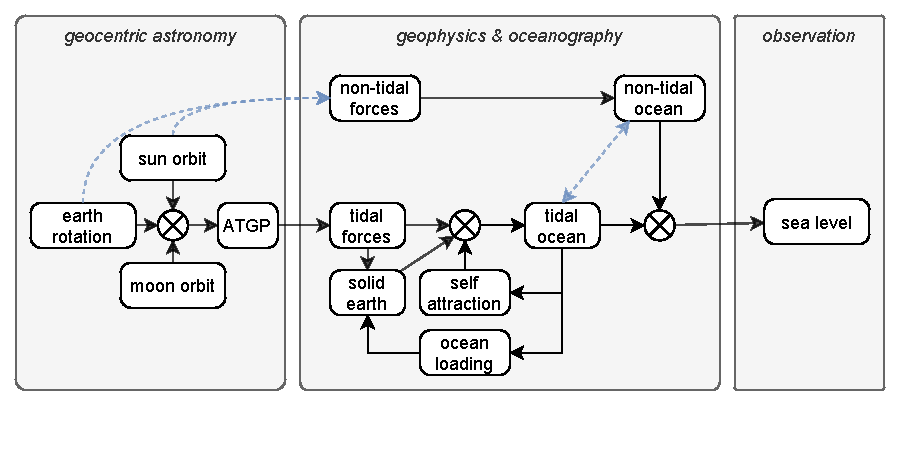
\includegraphics[width=\figwidthFull]{figures/diagrams/tidal_force_flowchart.pdf}
    \caption{Ocean tide flow chart (following Agnew \citep{Agnew:2011ub}.  Reference to the \ATGP{} is common to tidal analysis and prediction methods, whilst the treatment of tidal/non-tidal connections can differ markedly.}
    \label{fig:tideForceFlow}
    \end{center}
\end{figure}
%-----------------
Before expanding on the role of the tidal forcing, the recent work of \cite{10.1016/j.oceaneng.2020.107013} is worth mentioning.   Regardless of the finer details, this observation-based machine learning application to tide prediction is still founded on the connection between positional astronomy and sea level, but simply makes the connection more indirect by relying on easily accessible moon phase data.
%-----------------i
\subsection{Basic development of the \ATGP{}}  \label{sec:basic_potential}
The centrality of the tidal generating potential to sea level forecasting warrants further elaboration, in order to later explicate the manner in which conventional and dynamic sea level forecasts respectively represent tides. 

The \ATGP{} is a mathematical abstraction founded on a consideration of the classical gravitational field near the Earth surface. The temporal variations of gravity in the vicinity of this surface are developed as a function of the \emph{geocentric} relative positions of the celestial bodies.
For ocean tide applications, only the two celestial bodies, the moon and sun, are considered relevant on the basis of relative contribution to the perceived gravity field changes. It follows that the information required for computation of this lunisolar tidal potential is encapsulated in the celestial positions (ie ephemeris) of the moon and sun alone \citep{Agnew:2011ub}.


The full gravity field is defined as a scalar potential in space fulfilling the Laplace equation $\Delta V=0$ \citep[sec 5.3.1]{Urban:2013vl}.  The spatial field $V(\theta,\lambda,r)$ can be formulated in spherical geocentric (ie fixed earth) coordinates as a weighted sum of surface spherical harmonics. As a potential field, contributions from each mass element can be computed separately and linearly superposed.

The specific subset of $V$ attributed to the celestial bodies external to the Earth, but excluding components acting uniformly over the Earth's surface, is defined to be the tidal potential \ATGP{} or $V_T$.
The associated tidal acceleration at any particular point on the earth surface can also be thought as the vector difference between the direct attraction of each celestial body and the orbital acceleration about the Earth-Body barycenter \citep{Wenzel:1997kn}.


The subset $V_T$ of $V$ that is relevant to ocean dynamics is formulated in geocentric coordinates following the convention of \cite{Cartwright:1973em} hereafter \CTE{}, and more recent notation of \cite{Desai:2006wo}:
\begin{equation}
    \eta_{eq} = \frac{V_T(t,\theta,\lambda) }{g} = \sum_{n=2}^{\infty} \sum_{m=0}^{m=n} M_{nm} P_{nm}( \sin(\theta) ) \text{Re} \left [ c^{*}_{nm}(t) e^{im\lambda} \right ]
    \label{eq:VT}
\end{equation}
Where the potential is described only on an idealised spherical earth surface in terms of time, longitude $\lambda$ and latitude $\theta$, as a sum of functions described further below. 

$P_{nm}$ are the associated Legendre polynomials of degree $n$ and order $m$.  Writing $P_{nm}(\sin(\theta))$ gives the surface spherical harmonics.   Note that some other formulations may appear to differ due to use of a co-latitude coordinate.   
$M_{nm}$ are normalisation factors, that whilst not of direct interest here are noted to follow different conventions in some applications \cite{Anonymous:2004tm}.
Figure \ref{fig:VTmaps} provides a visualisation of the field and decomposition into components for a snapshot in time.

%-------------------------------
\begin{figure}[h]
    \begin{center}
    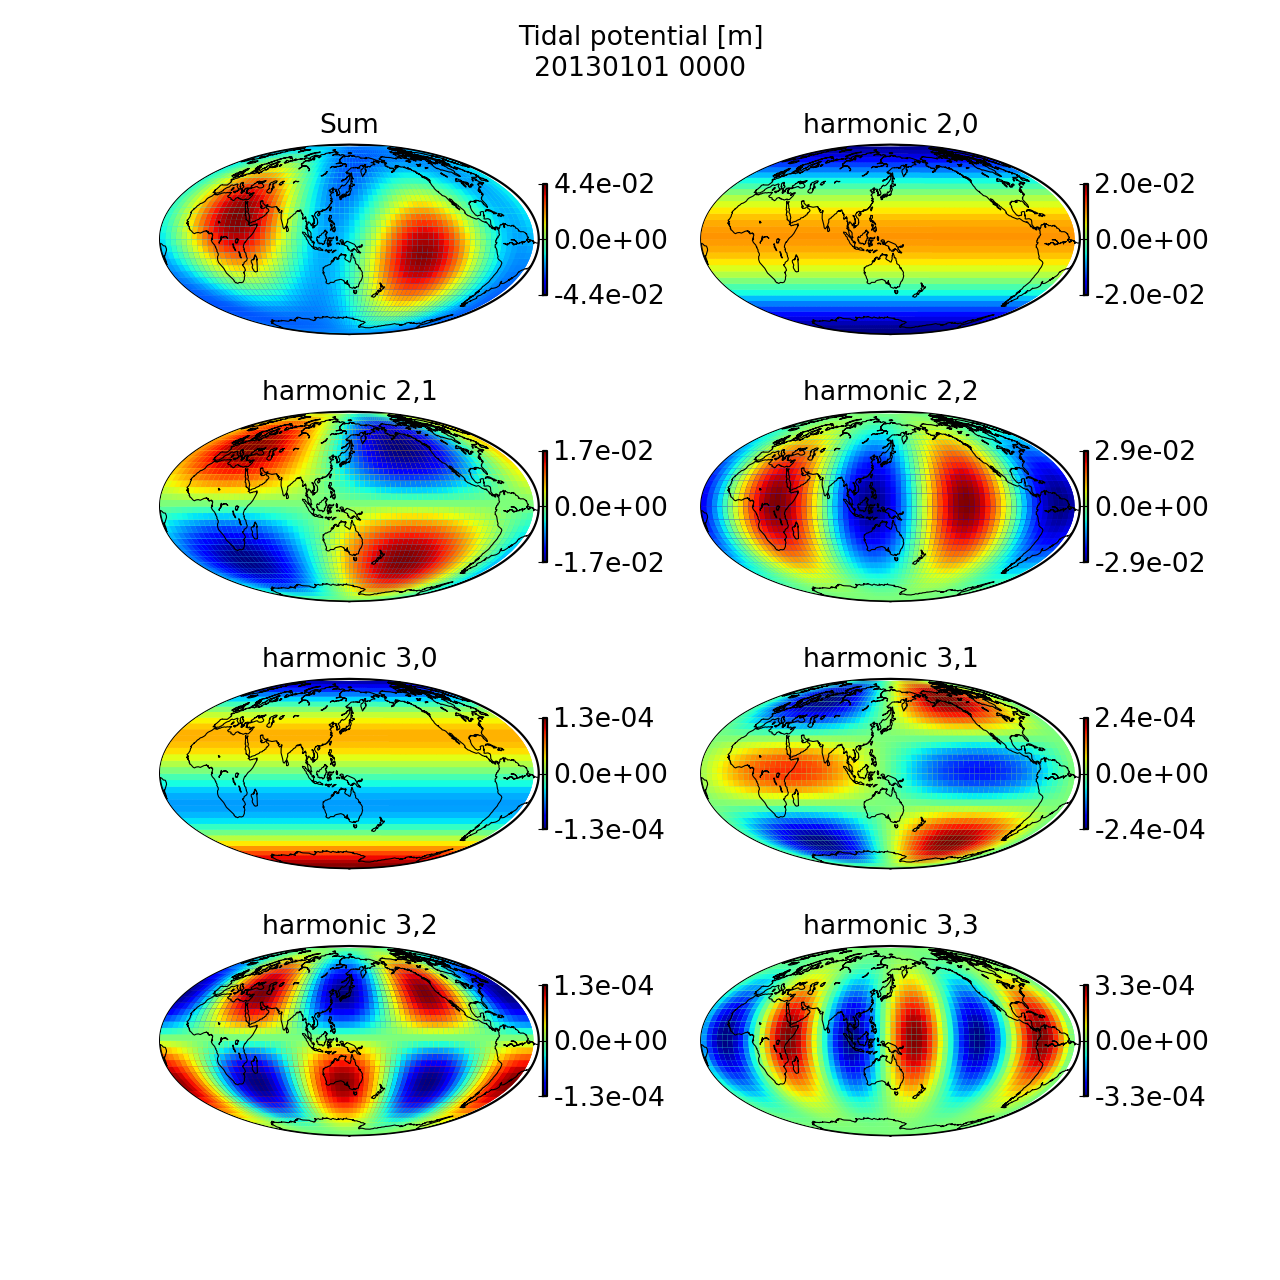
\includegraphics[width=\figwidthBig]{figures/maps/tidal_potential_spatial_20130101_0000.png}
    \caption{Snapshot of global $\eta_{eq}$ field illustrating spatial decomposition into spherical harmonics.  Note the wide variation of relative magnitude}
    \label{fig:VTmaps}
    \end{center}
\end{figure}
%-------------------------------
Equation \ref{eq:VT} It is conventional to refer to $V_T$ normalised by the standard value for Earth gravity $g$ as the \emph{equilibrium tide} $\eta_{eq}$.  Conveniently, $\eta_{eq}$ has units of height.  Writing the potential as an abstract height field $\eta_{eq}$ is common in the ocean literature as it can facilitate tidy formulations; for instance \cite[Eq 9.8.3]{gill1982atmosphere}.   Use of the term `equilibrium tide' can unfortunately be a source of miscommunication, inviting confusion with actual ocean elevations or some meaningful equilibrium ocean state - which it is not.


Equation \ref{eq:VT} represents very generally the spatial decomposition of a surface field over the globe.  Of itself, the formulation asserts nothing specific about the causation of the field.  It embodies no astronomy or ocean dynamics.

Practical implementation of \ref{eq:VT} requires choices regarding the set of harmonics $(n,m)$ to be included and the determination of the complex weights $c_{nm}(t)$.


In contrast to the thousands of harmonics utilised in high resolution gravity studies, for ocean tidal dynamics only a small set of $(n,m)$ is taken to be relevant.   The tidal subset is determined on the basis of relative magnitude and contribution of temporal variation at relevant scales.


Very generally, it is only the horizontal gradient $\nabla V_T$ that can effect the distribution of ocean mass.  And furthermore, only temporal changes in this horizontal gradient will effect the non-static ocean distribution. Subsequently degrees $n=0,1$ are not relevant to ocean tides.   This is represented in Equation \ref{eq:VT} by the lower limit $n=2$ of the outer sum.


For almost all ocean studies an upper limit of $n=2$ is taken to be sufficient, or at most $n=3$.  This choice is based on the rapid decline in relative magnitude with increasing $n$ for the luni-solar system - discussed below regarding Equation \ref{E:c}.



It may also be proper to exclude at least some of $(n,m) = (2,0)$ for many ocean tidal uses.  Specifically, by having no variation in $lambda$ this largely contributes to the 'permanent tide' associated with mean dynamic topography rather than temporal variations.  Treatment of $(n,m) = (2,0)$ is worthy of special attention and care with regard to each ultimate application.  One instance is that the relatively slow temporal variations are associated with the so-called long-period tides - which includes seasonal cycles.  Also, the need to ensure complementarity treatment of $(n,m) = (2,0)$ with regard to geoid models is discussed in \cite[section 5.3.3.2]{Urban:2013vl}.




All of the temporal variation of $V_T$ is contained in the time series of complex scalar weights $c_{nm}(t)$.\\
It is significant that the temporal variations of the \ATGP{} for the entire globe can thus represented by a small number of scalar timeseries - a single complex timeseries for each spherical harmonic included.  For the typical set of harmonics used for ocean tides $(n,m)=(2,1),(2,2)$ this represents a significant compression of spatial information.  The normalisation used in the determination of $c_{nm}(t)$ must be consistent with \ref{E:M}.\\

\begin{figure}[h]
\begin{center}
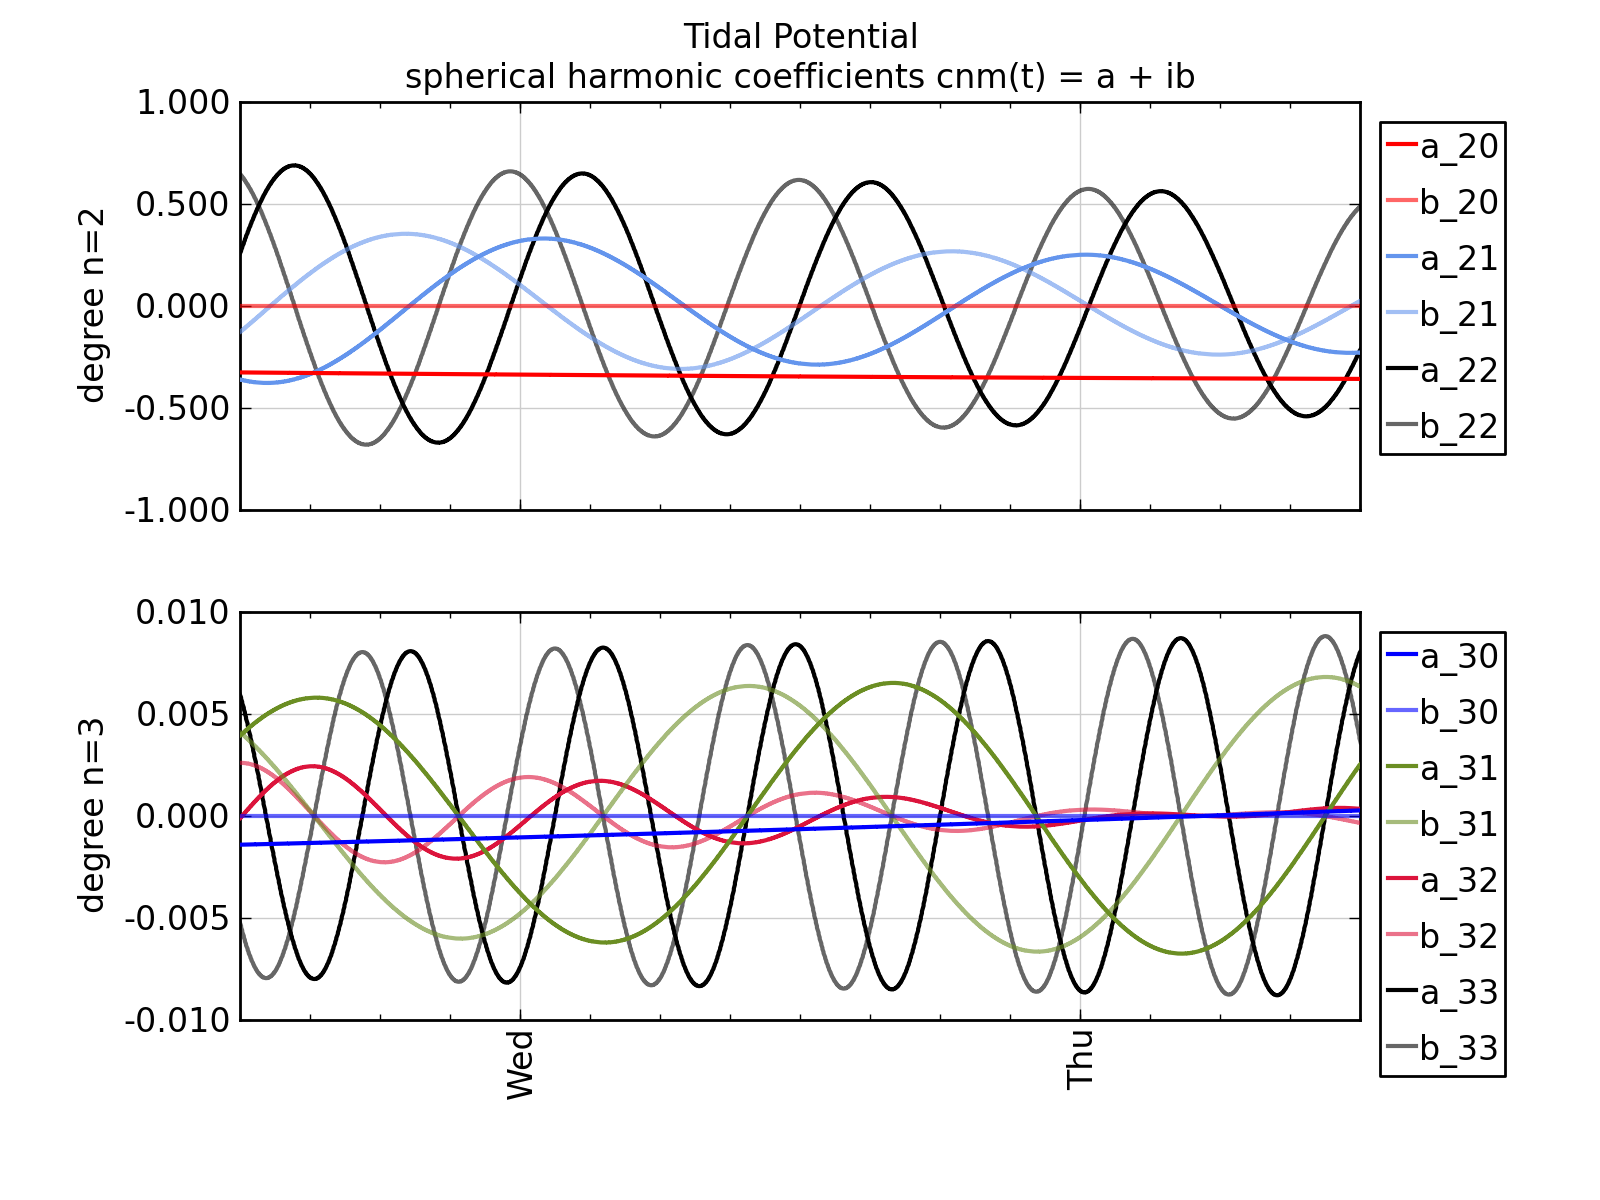
\includegraphics[width=\figwidthBig]{figures/plots/tidal_coeff_timeseries_2days.png}
\caption{Snapshot of time varying coefficients $c_{nm}(t)$.  In the upper panel, classification of $c_{2m}$ into long, diurnal and semi-diurnal `species' is evident.  Note the much smaller magnitude of higher degree harmonics.}
\end{center}
\end{figure}

The luni-solar coefficients are determined from the instantaneous positions of the Moon and Sun relative to the geocenter.  Such information is referred to as ephemerides \citep[Section 8.1]{Urban:2013vl}
Given the positions in the geocentric reference frame $\theta,\lambda,r$ for both Moon and Sun, the coefficients are:
\begin{align}
\label{E:c}
c_{nm}(t) &= a_{nm}(t) + ib_{nm}(t) \nonumber \\
          &= \sum_{b=\text{moon},\text{sun}}    \frac{4 \pi GM_{b}}{g r_{b}}  \frac{(2-\delta{m0})} {(2n+1)} \left(\frac{a}{r_b} \right)^n    M_{nm} P_{nm}( \sin(\theta_b) ) e^{im\lambda_b}
\end{align}

Note that $\theta,\lambda$ in Equation \ref{E:c} are equivalent to the geographic coordinates of the respective sub-body point at a given time. 
Where $\delta_m0 = 1$ for $m==0$ and $\delta_m0 = 0$ for $m \neq 0$.\\
Normalisation $M$ is given by Equation \ref{E:M}. The radial scale $a$ is conventional taken as the semi-major axis from the ellipsoidal georeference. 



The rapid decay of the scaling term $\left(\frac{a}{r_b} \right)^n$ with n is the basis for excluding higher degree harmonics from ocean tide applications.  In the case of the Moon, the magnitude of the $n=3$ potential field is more than 2 orders of magnitude smaller than $n=2$.  The associated force also decays, but not quite so rapidly due to the decreasing spatial length scales of the higher harmonics.  This decay is apparent in the colorbars of Figure \ref{fig:VTmaps}\\
The same relative magnitude argument is applied to neglecting more distant celestial masses from formulation of $\eta_{eq}$.



%-----------------%
\subsection{Phenomena included in the \ATGP{}}
\label{S:ATGP_extras}
The essential development of the \ATGP{} in Section\ref{S:basic_potential} is standard.  However, progressing beyond the basic development towards an ocean forecasting application raises several issues of significance that depend on the details of the application.\\


\underline{Solid Earth deformation and vertical reference.}  \\
The basic spatial perspective behind the development of the \ATGP{} is the thin shell approximation.  Geocentric coordinates are used.  This is appropriate for writing the potential in general form.  However, when considering the response of ocean dynamics, a vertical relative to the ocean floor is dynamically relevant.  There is a vertical movement of the ocean floor in geocentric coordinates associated with the \ATGP{} of comparable magnitude to the ocean tide which is quantitatively significant to dynamic models \citep{Hendershott:1981ub} and \citep[pp.336]{gill1982atmosphere}.\\
This elastic response of the earth can considered to be essentially instantaneous compared to ocean timescales.  Furthermore, the elastic re-distibution of mass associated with this 'earth tide' itself modifies the gravitational field.    By treating the Earth as "spherical, non-rotating, elastic, and isotropic" the solid body response can be encapsulated by a small number of dimensionless Love numbers \citep{Agnew:2011ub}.  In the present context each spherical harmonic degree has a single body tide Love number $h_n$ and `induced free space potential' Love number $k_n$ \citep[Sec 5.3.3]{Urban:2013vl}. This has the convenience of formulating the combined \emph{direct} effects of the solid earth response to the \ATGP{} as a modification to the magnitude of $\eta_{eq}$.  It is noted that ``the Love numbers for the diurnal tides differ from those for the semi-diurnal and long-period tides because of the free-core nutation resonance'' \citep{Arbic:2004wz}.\\
The conceptually related, but more complicated, effects of the moving ocean mass itself is discussed below.

\begin{equation}
\eta_{eq} = -(1+k_n-h_n) \frac{V_T}{g} \sim 0.7 \frac{V_T}{g}
\end{equation} 



\underline{Treatment of self attraction and loading.} \\
The tidal movement of ocean mass has an effect on the solid Earth, and reflexively on the gravitational potential acting on the ocean itself.\\
From an ocean modelling perspective, elastic compression of the solid earth due to the time varying mass of ocean is referred to as the `load tide'.  The effect of the moving distribution of ocean mass on the gravitation potential field is referred to as `self-attraction'.\\
Together these effects are lumped together as self-attraction and loading \SAL{}.  They are conceptually distinct from body tides in that \SAL{} is a reflexive function of the time varying spatial distribution of global ocean mass.\\
Similar effects that vary on tidal timescales are also associated with the time varying distribution of atmospheric mass as well land-based loading from ice,snow and soil moisture.  The value of explicitly distinguishing non-ocean \SAL{} in the context of ocean forecasting is not known, and no publications appear to address this in detail.  It is likely that practical evaluation of \SAL{} for ocean modelling implicitly accounts for some atmospheric effects - especially for the ocean tide associated with pressure forcing S1 and S2.\\



Similarly to body tide effects, it is possible to formulate \SAL{} as a scaled modification to the \ATGF{}.  This is very convenient, but known to be associated with significant inaccuracies \citep{Ray:1998jl}.  The present distribution of \MOM{} makes this so called `$\beta$' approximation.\\
An evaluation of intermediate methods to parameterise SAL is described by Stepanov and Hughes \cite{Stepanov:2004up}
In contrast to the $\beta$ scaling approximation, it appears to be quite reasonable to consider \SAL{} as separate pre-calculated body forcing rather than a scaling of $\eta_{eq}$. 
\begin{quotation}
SAL should be computed by convolution \dots with the Green's function for loading and self-attraction. Since this convolution smoothes out small-scale features, and since large-scale tidal elevations are now well determined over most	of the earth, SAL is in fact now reasonably well known, even where local details of tidal elevations and currents remain uncertain. \citep{Egbert:2002ug}
\end{quotation}




\underline{Time, polar motion and ephemeris.}\\ 
Diurnal Earth rotation and hence time UT1 are effected by tidal effects \citep[sec 8]{Anonymous:2004tm}.  In addition, conventional UT1 contains discontinuities at leap seconds is not strictly identical to ephermeris time.  For the purposes of ocean forecasting these variations are in general considered negligible and definitions of time are treated as unproblematic.\\




A special case is the \underline{pole tide}. Geocentric coordinates align the polar zenith approximately with the Earths axis of rotation. However, there are continual variations of alignment from the reference axis described by theories of precession and nutation and in general referred to as `polar motion'.   More generally, any changes in the Earth's instantaneous rotation vector can be associated with changes in the gravity field  experienced in surface fixed geocentric coordinates.\\
\begin{quotation}
Polar motion of the Earth is almost completely described by two harmonic variations of the location of the instantaneous rotation pole with respect to the mean rotation pole: an elliptical motion at an annual period, and an almost circular motion at a period of 14 months. The 14-month variation is a free mode of the Earth referred to as the Chandler wobble and has amplitudes that vary with time. \citep{Desai:2002ev}
\end{quotation}
The gravitational effect due to polar motion can be formulated similarly to the \ATGF{} as a potential field decomposed into spherical harmonics.
Pole tide effects are included as corrections to altimetry products, but are ignored in standard tide table production.\\
Another phenomena effecting Earth rotation is the Free Core Nutation (FCN).  For the present ocean tidal purposes the FCN will be considered relevant only with regard to the solid earth tides.  The FCN is a factor in defining the  Love numbers in the diurnal band.   Related to this, Desai and Wahr note that the definition of the K1 $[1 1 0 0 0]$ input amplitude used for solid earth tide algorithms can be inappropriate for ocean applications if compensation for the effects of the FCN resonance are included\cite{Desai:1995je}.



The formulation of the tidal potential in Section\ref{S:basic_potential} involved only the instantaneous relative positions of the Earth-Moon-Sun system.   These positions are taken from an ephemeris.  In practice, there are two broad classes of ephemeris; analytical and numerical \citep{Wenzel:1997kn}.\\
An analytical ephemeris provides the relative positions of the Moon and Sun via relatively simple polynomial relations, optimised for a given epoch.  Such analytic ephemeris have been commonly employed for ocean tide studies.   Analytic ephemeris were used initially for computational necessity and more recently for computational convenience.\\
For modern astronomical purposes numerical ephemerides are now standard.  Prior to 1984 standard ephemeris were based upon \emph{theories}\cite[sec 8.1]{Urban:2013vl}, whereas contemporary ephemeris are created in a manner analogous to \NWP{} or operational oceanography: dynamical equations are integrated into the future, after initialisation via assimilation of past observational data.\\
At the time of writing, the `current best estimates' for the orbits of the Moon and planets is DE421 \citep{Folkner:2008wm}.   The snapshot visualisation shown in Figure \ref{fig:VTmaps} have been calculated based on application of Equations \ref{E:M} and \ref{E:c} to output of DE421 utilising the software tools provided by NASA \cite[p]{Anonymous:vo}.\\
Any differences between modern ephemeris over ocean forecasting timescales are expected to be very small.   However, an evaluation of such differences may be a relevant undertaking in the body of this work - in particular between the best estimate and any analytic formulations employed in an ocean model.



%-----------------%
\subsection{Special role for temporal variations}
The \ATGP{} varies in time.  Variations over forecasting timescales of several days are most relevant to the present discussion, though it worth noting that much longer astronomical timescales play a role in quantification.\\
Just how these temporal changes are formulated is fundamental to the different tidal methods.   In short, the temporal changes can be written in time-space or frequency-space.\\



All the time variation in Equation \ref{E:V_T} is contained in the coefficients $c_{nm}(t)$.  A tidal method based on $c_{nm}(t)$ derived from a numerical ephemeris could be said to be \emph{direct}.\\
A direct application of $c_{nm}(t)$ is at face value conceptually consistent with modern numerical ephemeris.\\



Alternatively, transformation of $c_{nm}(t)$ in to frequency-space is the basis of many tidal methods.   The highly clustered frequency content of $c_{nm}(t)$ renders this transformation particularly useful.  The spectral content of $c_{nm}(t)$ is not strictly a stationary line spectrum but is very nearly so for relevant timescales.\\
Transformation of $c_{nm}(t)$ into frequency space is the basis for \underline{harmonic developments} of the \ATGP{}. Whilst there have been different approaches to performing this development, the common representation is given in Equation \ref{E:harmonic} following \citep{Desai:2006wo} and \citep[Eq 13]{Cartwright:1971iz}.\\
As with much of the tidal nomenclature, the possible confusion of the distinct concepts of `harmonic decomposition' with `harmonic analysis' is worth noting.
\begin{equation}
\label{E:harmonic}
c_{nm}(t) = \sum_{k} H_{nmk} e^{-i( t\theta_{nmk})} = \sum_{k} H_{nmk} e^{-i( t\omega_{nmk} + \beta_{nmk})}
\end{equation}


The index $k$ represents a discrete series of hundreds of tidal components.  Each component is associated with a discrete point in complex frequency-space with amplitude $H$, frequency $\omega$ and phase $\beta$.
It is important to emphasise that Equation \ref{E:harmonic} does not represent a Fourier series.  The sequences of frequencies $\omega_{nmk}$ are derived from the orbital motions of the Earth-Moon-Sun system and do not result in an orthogonal set of sinusoids.\\


Doodson \citep{Doodson:1921kt} introduced a novel and influential system of notation for specifying $\theta_{nmk}$ based on his laborious harmonic decomposition of $V_T$ using Brown's lunar theory.  In the Doodson formulation, all the relevant astronomical information is summarised by code of 6 small integers; together called the `Doodson number' or `argument numbers'.   Each position in the code is associated with an fundamental astronomical concept as summarised in Table \ref{T:doodson}.  Doodson codes are in common use across the tidal literature and provide the only useful means of describing tidal components beyond the very small number associated with traditional Darwin names M2, K1, O1, S2 etc.\\
There has been some variation of conventions with regard to the exact formulation of Doodson numbers.  One such detail is the avoidance of negative integers in the code by the addition of the arbitrary constant 5 to all integers except $d_1$.   A less common variation involves the use of solar-hour in place of lunar hour $\tau$.  In the context of ocean tide prediction, the attribution of codes to harmonics is not consistent, but this is discussed in later sections. \\
In essence the Doodson codes provide a compact unique specification, or in practice \emph{definition} of frequencies relevant to tidal methods.


\begin{table}[htp]
\caption{Doodson astronomical arguments.  Small integer combinations of these six numbers $d_1 d_2 d_3 d_4 d_5 d_6$ are used to classify tidal components.}
\begin{center} 
\begin{tabular}{|c|c|c|}
\hline
Description                            & Argument          & Period\\
\hline
Mean lunar hour                        & $\tau$            & $\sim$ 1 day      \\
Moon mean longitude                    & $s$               & $\sim$ 27 days    \\  
Sun mean longitude                     & $h$               & $\sim$ 1 year     \\
Longitude of lunar perigee             & $p$               & $\sim$ 8.85 years \\
Negative longitude of mean lunar node  & $N^\prime$        & $\sim$ 18.6 years \\
Longitude of Sun mean perigee          & $p_1$             & $\sim$ 20000 years\\
\hline
\end{tabular} 
\end{center}
\label{T:doodson}
\end{table}


Equation \ref{E:doodson} gives the angular argument for a single tidal component $k$ as a function of the 6 astronomical arguments.   As discussed above, the astronomical arguments embody an analytical ephemeris for the Moon and Sun rather than a direct numerical description of these positions.  Polynomial functions of time can be used to estimate each of the 6 arguments close to a given epoch.  The phase adjustment $\delta$ is a convention applied such that the each term in \ref{E:harmonic} is written as a cosine, rather than the mixture of sine and cosine terms that naturally follow from the underlying spherical harmonics.

\begin{align}
\label{E:doodson}
\theta_{nmk}  &= \left[ d_1 , d_2 , d_3 , d_4 , d_5 ,d_6 , \delta(n,m)  \right] \cdot \left[ \tau , s  , h , p , N^\prime , p_1 , \frac{\pi}{2}   \right]   \\
          d_1 &\equiv m \nonumber \\
              & \mbox{ (nb ignoring integer offset 5 often added to $d_2d_3d_4d_5d_6$)} \nonumber
\end{align}

\begin{equation}
\delta(n,m)  =     \begin{array}{ll}
                    1 & \mbox{if $n+m$ odd}  \\
                    0 & \mbox{if $n+m$ even} 
                    \end{array}             
\end{equation}


%-----------------%
\subsection{Ocean as an LTI System}
\label{S:LTI}
With historical hindsight it could be said that the success of tidal sea level prediction have been based on treating the ocean as a linear time invariant (LTI) system driven by the \ATGP{}.\\
In essence, temporal variation in the \ATGP{} is an input that the LTI maps directly to an predicted ocean response.  Once such a time invariant `black box' for the ocean has been characterised,  accurate astronomical predictions can be mapped to an ocean prediction.  The details of how the LTI system is characterised and implemented distinguish the variants of tidal analysis and prediction.\\




Two important aspects of this broad approach were introduced in the late 1700's by Laplace \cite[chpt 7]{Cartwright:2000tt}:
\begin{itemize}
\item spectral banded-ness of $V_T(t)$ (classified into diurnal, semi-diurnal and long species) and the value of a stationary frequency perspective;
\item semi-empirical analysis to characterise the stationary frequency-space outcome of complex global hydrodynamics. 
\end{itemize}


\BoxBegin
Modelling the ocean as an LTI system in this manner necessarily takes a frequency-space perspective and relies on stationarity (time invariance). Jay and Kukulka \citep{Jay:2003bj} suggest that that the long history and apparent value of this perspective has $\dots$
\begin{quotation}
solidified an opinion that tidal time series (particularly those of surface elevation) are basically stationary, with non-stationary components frequently being regarded as meaningless `noise'.    
\end{quotation}

In fact, as discussed in Section \ref{SS:semantics}, time stationarity is essential to the \emph{definition} of `tidal' in most operational settings.
\BoxEnd


\begin{align}
    c_{nm}(t)       \Rightarrow & \fbox{Global Ocean} \Rightarrow \mbox{observed response}                \nonumber 
\end{align}


Time invariance of the LTI in frequency-space means that each input component maps directly to an output response at the same frequency, characterised by a amplitude and phase transformation.   As the LTI characteristics are identified via semi-empirical methods,  the complex dynamics are hidden within the `black box' and are largely irrelevant.\\
The core of such a tidal model is schematically shown as a mapping at each distinct tidal frequency:

\begin{align}
\label{E:LTI}
H_{k}(\theta_k) \Rightarrow & \fbox{empirical LTI system} \Rightarrow \mbox{tidal ocean $f(\theta_k)$}  %\nonumber
\end{align}

Although the empirical determination of the LTI model largely ignores intervening dynamics, the literature investigating the natural modes of the ocean provides a relevant backdrop.  Given the picture of a LTI system forced by frequencies that are close to resonance, empirical fitting can be sensitive to details.
\begin{quotation}
By an unfortunate coincidence, the size of the earth, the depth of the ocean, and the rate of earth rotation are such that the frequencies of the free modes of ocean oscillation are intercalated with the frequencies of the tide-generating consitituents.\citep{Groves:1975ky}
\end{quotation}



In practice, details and embellishments built into tidal methods lead to variations regarding the precise definition of a reference input signal and characterisation of the LTI system.   Following Munk and Cartwright \citep{Munk:1966ts} there are three foci for these complexities:
%\begin{inparaenum}[(i)]
\begin{itemize}
\item the background spectral continuum of ocean variation, 
\item non-gravitational phenomena that can be considered tidal and 
\item non-linear interactions.   
\end{itemize}
%\end{inparaenum}
The manner in which the three `interesting effects' are incorporated distinguishes between the two primary methods of tidal sea level prediction discussed in Section \ref{S:formalisms}.



As an aside, the nomenclature LTI is taken from engineering control theory.   It does not here refer to the historically influential Liverpool Tide Institute.


%-----------------%
\subsection{Tidal Harmonics and Formalisms}
\label{S:formalisms}
Note the simple fact that ``\textit{many organizations have developed their own methods of tidal analysis}''\citep{IOC:2005tj}. 

There is no unique approach to implementing the LTI concept of ocean tide prediction.   The different approaches are variously referred to as `methods' or `formalisms' and at a higher level share the LTI system model discussed above.  In very broad terms there are basically two categories: harmonic methods and response methods.   Within each categories there are variations that are more or less significant depending on context. 

TBC
``\textit{Standard harmonic methods demand little accuracy in the harmonic amplitudes of the [tidal] potential, since they use only the frequencies at which the larger amplitudes appear, and certain details on which to base nodal corrections}''\cite{Cartwright:1973em}

Within operational authorities, tide prediction is practically synonymous with harmonic methods.  These have an especially long historical legacy in both theoretical and applied settings \citep{Cartwright:2000tt}\citep{Parker:2007wq}.   Harmonic methods of sea level prediction are very successful and important and will continue to be so, regardless of other advances.  Most notably, harmonic analyses based on tide-gauge observations are thoroughly embedded in operation centres and the wider economy.   In Australia, this conventional role is embodied by the official promulgation of the  Australian National Tide Tables \ANTT.  These tables are required by law to be carried by many marine vehicles and have broader ramifications for uses such as cadastral definitions.\\
There are several different schools of convention that lead to various incompatabilities between operational centres. \\
At its foundation, harmonic tidal analysis and prediction characterises the LTI system via a finite set of amplitude and phase terms that are identified empirically.  Equation \ref{E:cos} shows the LTI model with constant amplitude $A_k$ and phase lag $g_k$, other terms are discussed below.  This situation is illustrated by the following simplistic assertion from the Australian Tide Manual \citep{PCTMSL:2009vy}:
\begin{quote}
The purpose of tidal analysis is to represent the water level or current time series by a set of harmonics, or sine waves, each of them having a specific amplitude and phase.
\end{quote}

\begin{equation}
\label{E:cos}
\eta_{tide}(t) = \sum_{k} f_k A_k \cos ( t.\omega_k + g_k + u_k)
\end{equation}


Significantly, the harmonics involved cannot be the full set of tidal frequencies arising from the decomposition $c(t) = \sum_{k} H_{k} e^{-i( t\theta_{k})}$.  Rather, for practical reasons the set is on the one hand truncated to a subset of `constituents', and on the other is augmented with additional `compound' or `overtide' frequencies.  Many details of implementation flow from these deviations from the simple LTI schematic \ref{E:LTI}.  Before discussing in the more detail, the main elements of harmonic analysis and prediction are summarised as follows: 
\begin{itemize}
\item reference input written as the harmonic equilibrium tide at Greenwhich $\eta_{eq}(t) = \sum{k} A_{k} e^{-i( t\theta_{k})}$;
\item determination of LTI model as a discrete set of constants via empirical projection of a timeseries of sea level observations onto a discrete set of harmonic functions;
\item conventions accounting for unresolved tidal frequencies; 
\item synthesis of deterministic tidal timeseries (referenced to astronomical timing in $\eta_{eq}$) valid only at the observation location. 
\end{itemize}

The practical value of harmonic methods reflects the special significance and \emph{predictability} of sea level variation occurring at tidal frequencies.  This value does not rely on explicitly describing ocean dynamics.  In fact, it is asserted that the \emph{absence} of fluid dynamics is a key strength of harmonic methods.   Harmonic analysis is a specialised method of statistical pattern fitting that fundamentally requires historical observations at the place of interest.   A record of historical observations at one place is essentially all that is required, with no need for spatial information or any additional inputs whatsoever. 



\begin{figure}[!h]
	\centering
	%\subfloat{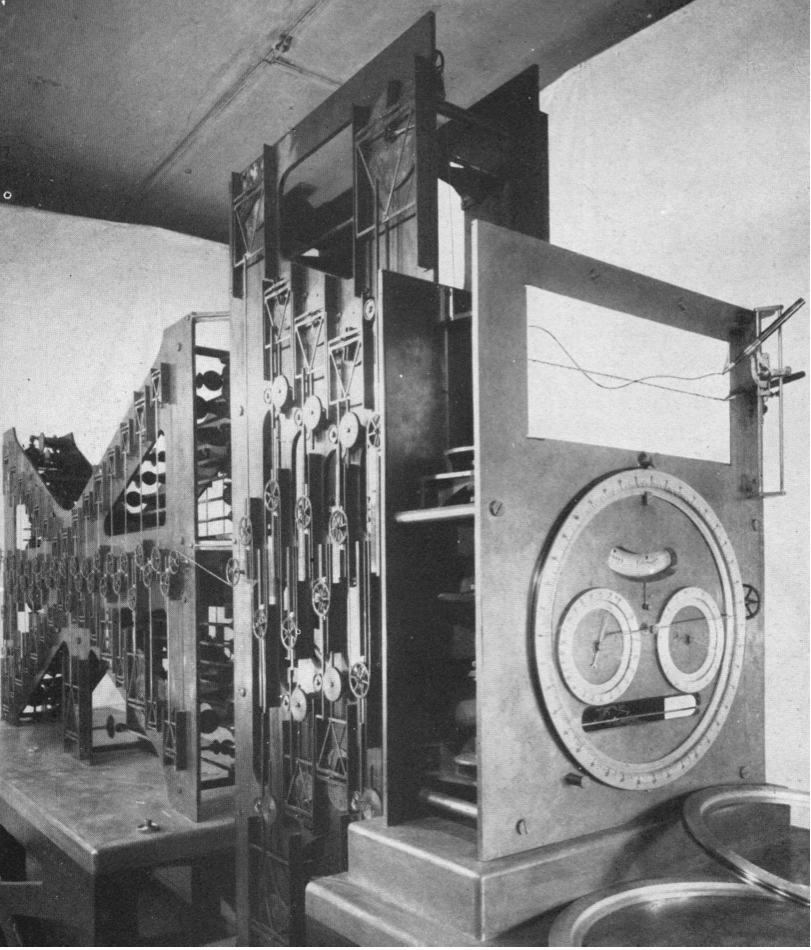
\includegraphics[width=50mm]{figures/images/HarrisFischer_tide_machine_ParkerFig1p1}}
	%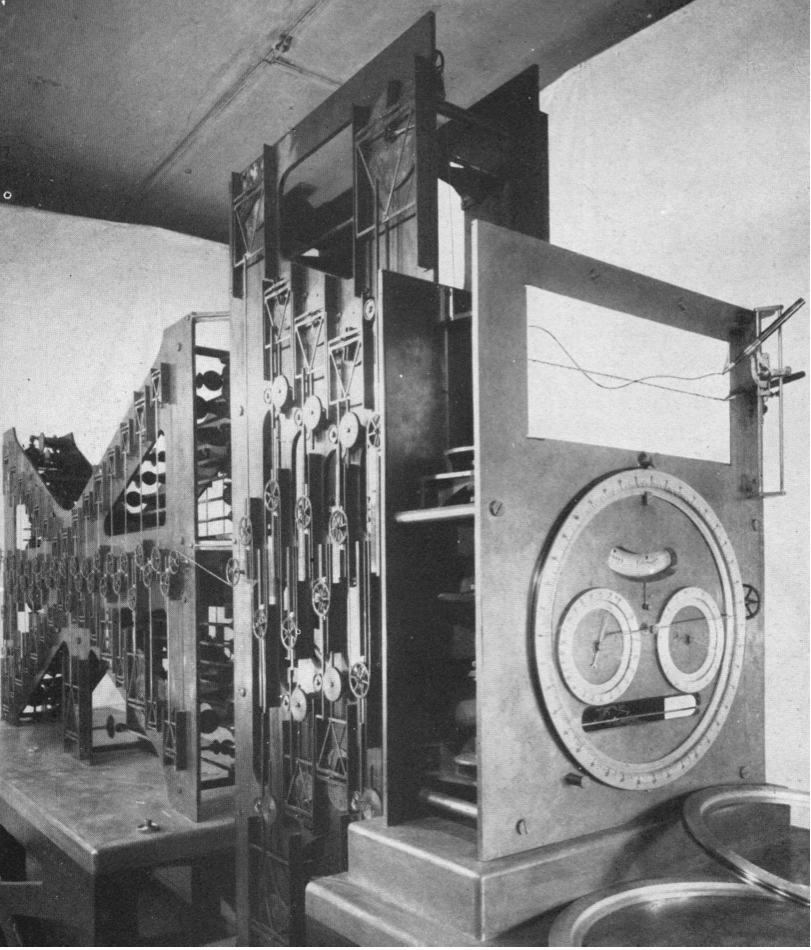
\includegraphics[width=50mm]{figures/images/HarrisFischer_tide_machine_ParkerFig1p1}
	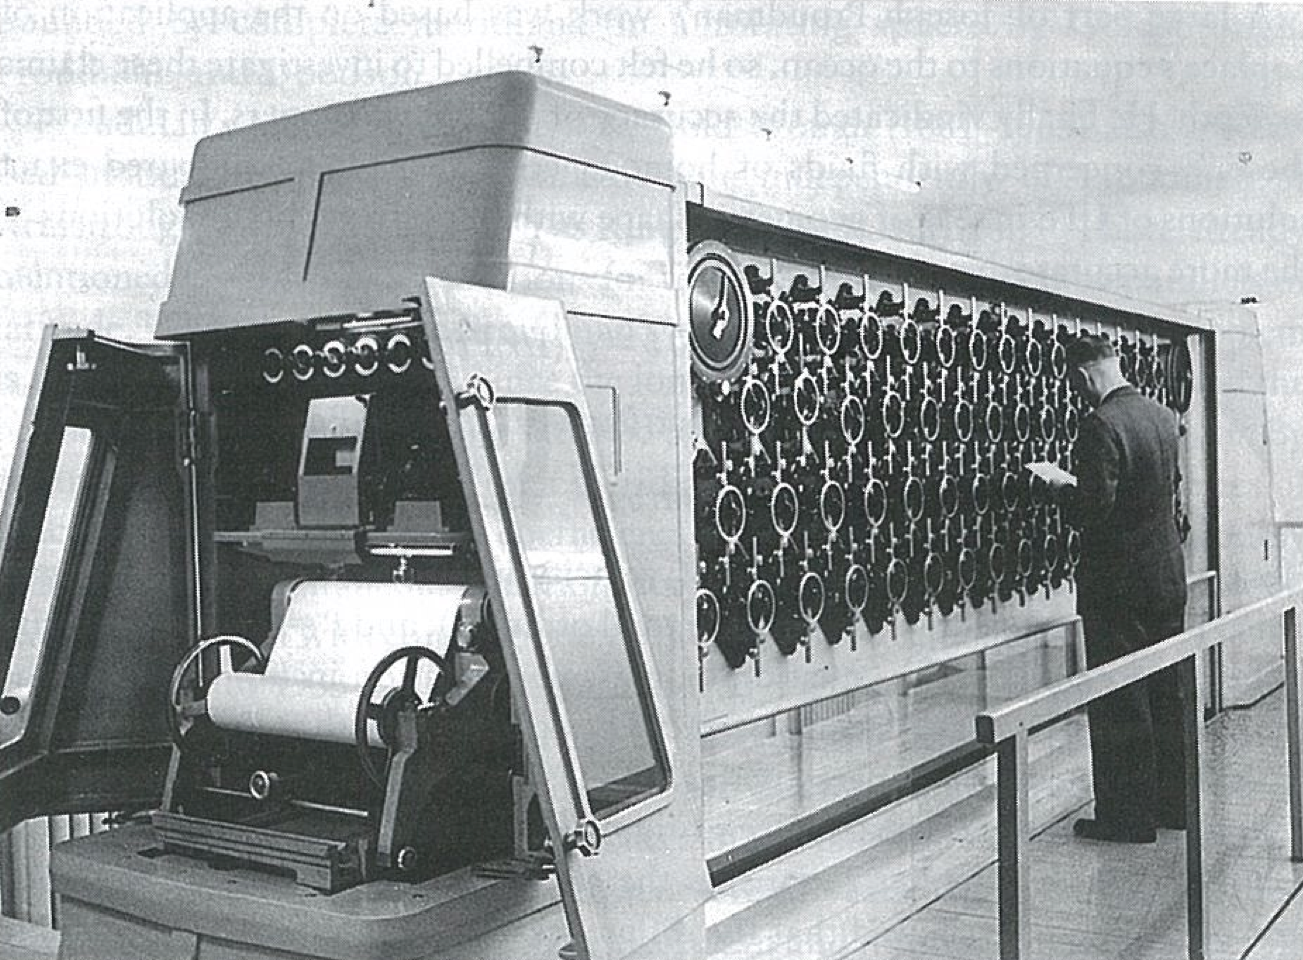
\includegraphics[width=50mm]{figures/images/DHI_machine_cartwright_fig11p2.png}
	\caption{Harris-Fischer tide machine circ. 1912 \protect{ \citep{Parker:2007wq} }}
	\qquad
	%\subfloat{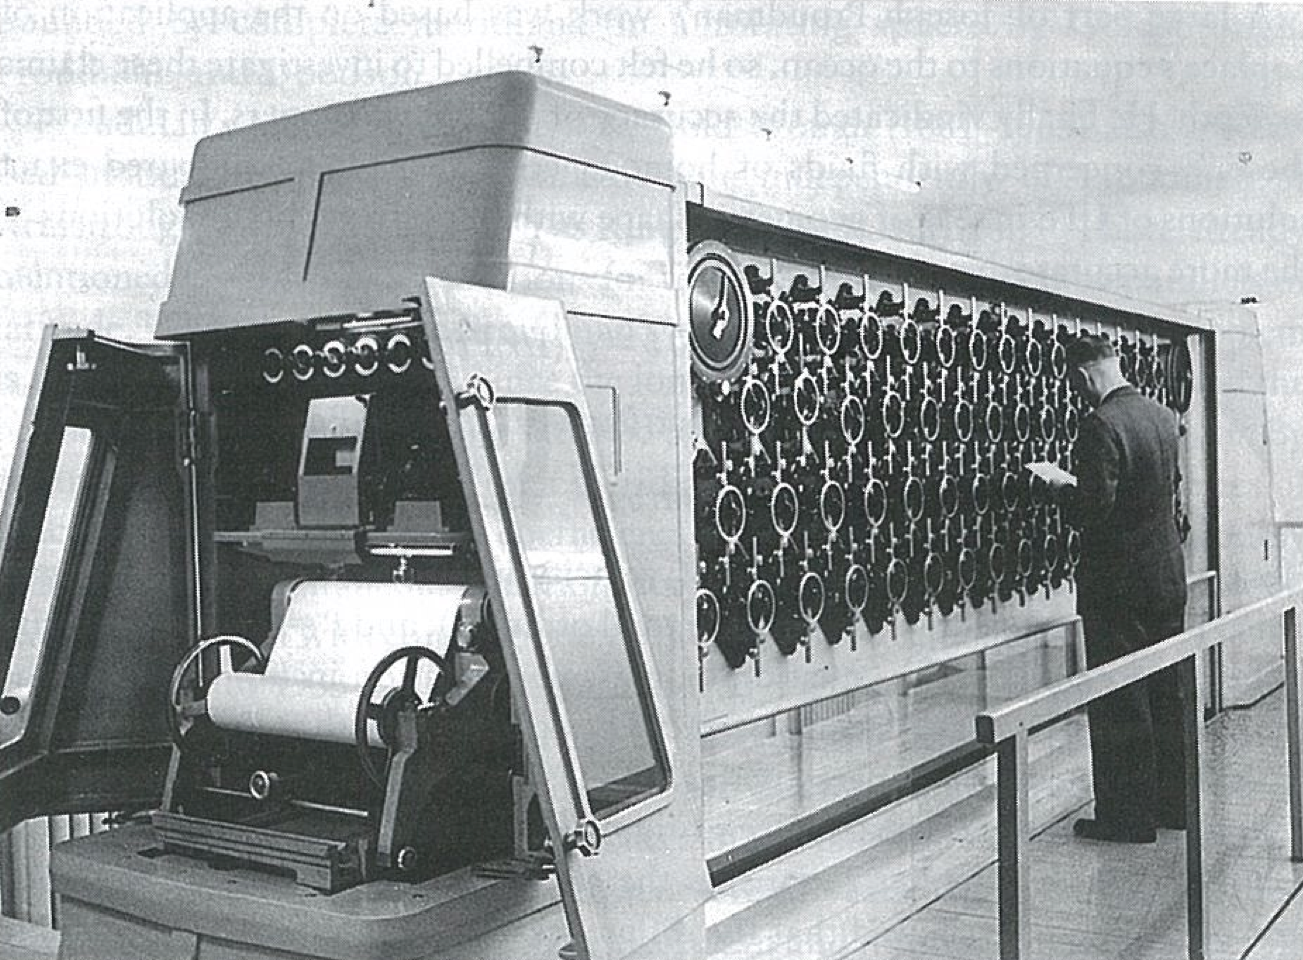
\includegraphics[width=50mm]{figures/images/DHI_machine_cartwright_fig11p2.png}}
    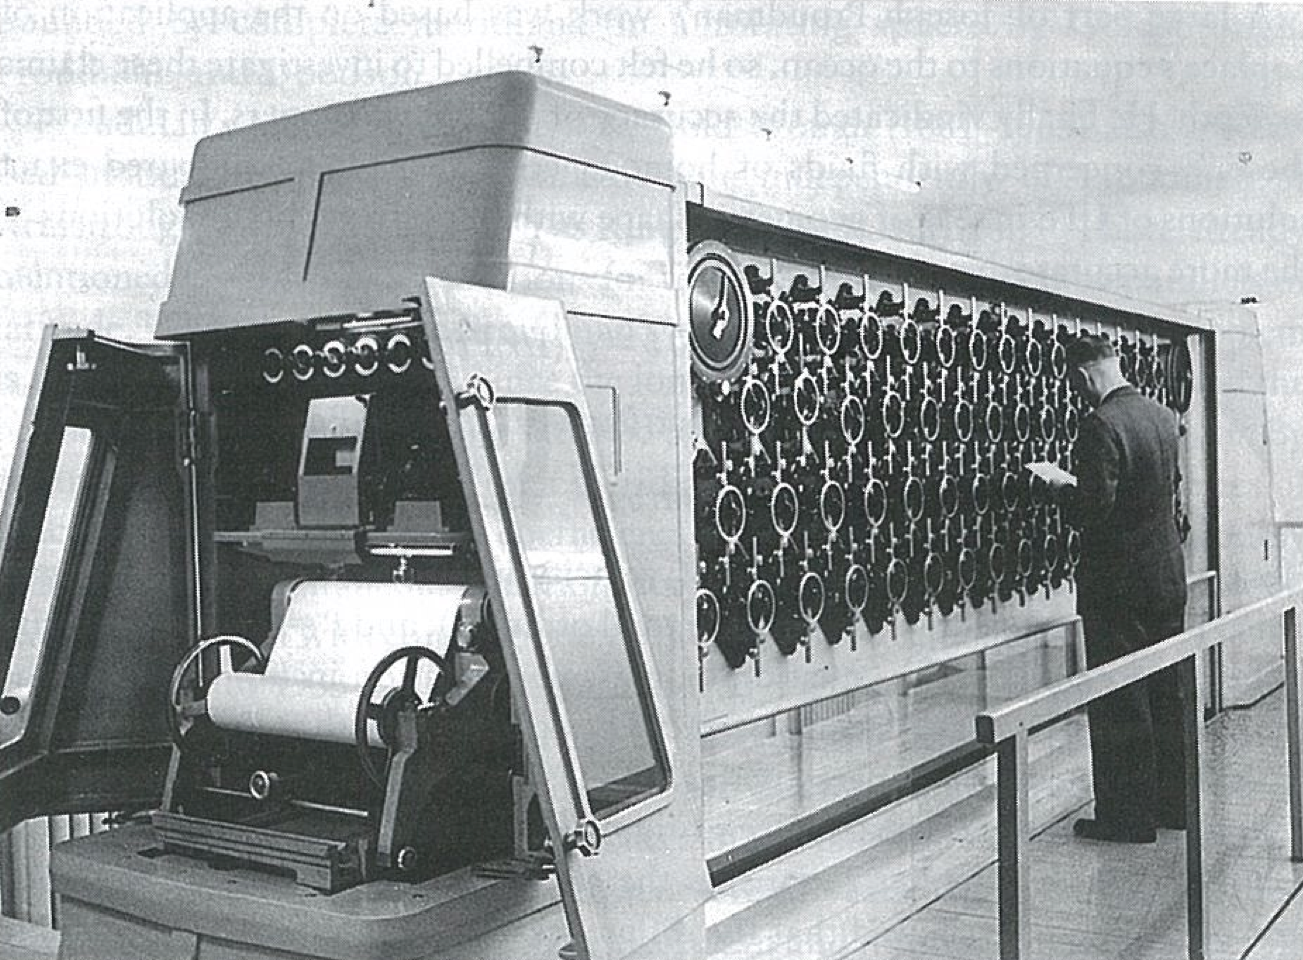
\includegraphics[width=50mm]{figures/images/DHI_machine_cartwright_fig11p2.png}
	\caption{Gezeitenrechenmaschine at DHI circ. 1940 \protect{ \citep{Cartwright:2000tt} }}
	\caption{Analogue tide machines embody harmonic prediction.  A finite set of fixed constants are dialled up for a port, and the handle turned to generate a prediction timeseries.}
	\label{fig:tide_machines}
\end{figure}


For almost all ocean-exposed locations, harmonic analysis can reduce the majority of sea level variance in a long observational timeseries to a remarkably short list of numbers - typically mapping several thousand values to a few dozen\citep{Flinchem:2000kp}.  Moreover, harmonic analysis isn't just an instance of data compression but can provide \emph{predictive} skill across lead times of many years.\\



In linear algebra terms,  a harmonic analysis can be formulated as an overdetermined inverse problem:
\begin{equation}
\label{E:Axb}
\M{A} \V{x}=\V{b} 
\end{equation}
Where $\M{A}$ is a matrix of tidal timeseries basis functions, $\V{x}$ is the analysed tidal solution and $\V{b}$ is an observational record. Importantly, the tidal basis functions are \emph{not} a Fourier basis.   The tidal basis is developed from the combination of the harmonic decomposition of $\eta_{eq}$ and a series of conventions.  The resulting basis is neither orthogonal nor complete.  The core assumption of stationarity for the finite series of basis functions is equivalent to an assumption that the basis has infinite span in time. \\




% harmonic complications
Pragmatic application of the harmonic formalism to real-world data has given rise to many conventions and work arounds, often perceived as opaque and arcane. \\

For instance, observational records are finite and typically of duration less than a harmonic analysis would nominally require.  Given the close clustering of tidal lines in frequency-space, Equation \ref{E:Axb} can be poorly conditioned for inversion.  Subsequently, practical procedures for tidal analysis must specify which frequencies to include in the basis set and then somehow account for the effects of unresolved frequencies\cite{Foreman:2009bg}.   \\
Typically arguments regarding the relative magnitude of the harmonic components of $\eta_{eq}$ are used to prioritise candidate frequencies for inclusion. Similarly, additional constants can be inferred rather than taken directly from the inverse solution, using assumed relationships from either $\eta_{eq}$ or previous or nearby analysis. \\
By convention, the effects of clusters of unresolved tidal frequencies are represented by modulation of the basis functions in relationships assumed to map from $\eta_{eq}$.  In equation \ref{E:cos} the modulation terms are included as $f_k$ and $u_k$. These are most common called `nodal corrections', due to close spectral spacing associated with the the lunar nodal regression (differences in $\omega_k$ of about $fract{1}{18.6}$ years.  Following Godin these very same terms are more informatively called `satellite modulations' by some authors (eg \citep{Foreman:2009bg}) in recognition that the modulation of a constituent term by a very closely spaced spectral cluster arises from terms other than $d_5$. Interestingly, modification of the tidal basis functions by nodal factors renders the analysis to be no longer strictly `harmonic' in that the basis does not consist of proper sinusoids.\\





%% non gravity
The occurrence of non-gravitational influences of sea level at tidal frequencies is a significant detail.   Non gravitational phenomena contribute to all three of Munk and Cartwright's \emph{interesting} effects cited above.  The inversion of Equation\ref{E:Axb} is a data-fitting exercise that cannot distinguish dynamical cause.  In particular, the presence of non-astronomical forces with frequency content at or very near that of the \ATGP{} can and does project onto the solution for $x$.\\
To the extent that the non-astronomical phenomena are regular enough to be predictably periodic, inclusion within the LTI model is can be to the benefit of a tide prediction.   On the other hand, effects that are not perfectly aligned to the \ATGF{} conflict with the fundamental LTI model and necessarily present an additional risk to forecast skill.\\
For instance with seasonal phenomena.   The harmonic decomposition of $c_{nm}(t)$ provides two relatively tiny signals at periods of 1 and 0.5 years - conventionally termed Sa and Ssa.  Despite the small amplitudes in $\eta_{eq}$ there are powerful seasonal variations in ocean observations that project onto the Sa and Ssa tidal components.   This is well recognised and `...whether the calculated values of Sa and Ssa are used or not, becomes almost a philosophical question, based on ones application' \citep[p122]{Parker:2007wq}.   Related terms that reflect seasonal modulation of semi-diurnal components can also included be included in standard harmonic analyses (eg H1 and H2 in Foreman schedule \citep{Foreman:1977ua})\\
Perhaps more significant methodologically, is the case of diurnal and semidiurnal sea level signals driven directly by \emph{meteorology} rather than the \ATGP{}.   The tidal frequencies denoted S1 and S2 are a prominent case in point.  For instance, Ray and Ponte \citep{Ray:2003ui} evaluate \NWP{} representations of \emph{barometric} tides at these frequencies with implications for oceanographic processes.  Treatment of S1 and S2 in tidal sea level predictions is a point of difference between the harmonic and response methods.  The later going so far as to invoke a distinct input function in the form of a `radiation potential'.    The response approach is now discussed in more detail. 





% response methods
The \underline{response method}, and it's variations, form the primary alternative to the conventional techniques of harmonic analysis.   This consists of a generalised implementation of the LTI model, in which the ocean response to \emph{any} input sequence is characterised by a stationary `admittance' function.  The terminology was introduced by the influential paper of Munk and Cartwright \citep{Munk:1966ts}, which was apparently motivated by an application of Ockam's razor to the highly evolved historical baggage of harmonic methods.   Godin \citep{Godin:1991vx} describes the response method as `cross spectral analysis'; a LTI model is inverted from comparison of the input and output timeseries.   Whereas harmonic methods evolved well before the availability of machine computers, the response method relies on computational signal processing with discretely sampled and finite length time series. \\
A response analysis aims to empirically characterise the LTI as a complex-valued transfer function on the basis of output coherence with the input/s. 
\begin{quotation}
The goal of any response formalism is to accurately predict the ocean tides by an optimum smooth function, realising that the ocean tides are mostly, although not completely, predictable.
\end{quotation}

Note that the outcome of a response analysis is not a single admittance curve, but rather a small number of distinct curves; typically the semi-diurnal, diurnal and long-period tides associated with degree-2 spherical harmonics $(n,m)=(2,2),(2,1),(2,0)$.\\
Smoothness of $Z(\omega)$ within each distinct tidal band is a core principle behind methods for determining admittances.  

\begin{align}
\label{E:response}
g(\Delta t) + \dots &\Rightarrow & \fbox{empirical admittance curves $Z$} &\Rightarrow & \mbox{$\eta(\Delta t)$}  %\nonumber
\end{align}

Once determined, admittance curves map a tidal input timeseries to an output timeseries.

% admittance
\begin{equation}
\label{E:Z}
\eta(t) = \sum_{n=2}^{3}\sum_{m=0}^{n}\sum_{k} H_{nmk} \text{Re} \left[ Z_{nm}(\omega)^*e^{-i(t\theta_{nmk})} \right] 
\end{equation}


The presence of incoherent noise in the observational timeseries means that determining $Z$ is not simply the matter of division in frequency-space.\\



In order to distinguish coherent signal from incoherent noise, Munk and Cartwright introduce the \emph{convolution formalism}. The convolution technique exploited the band-concentration of tidal spectra into semi-diurnal, diurnal and long period species and the associated assumption of \emph{smooth} admittances within each of these bands.  A complex-valued admittance $Z(i\omega)$ is fitted separately to each band-limited species via a convolution operation in time-space. 
Inversion of a smooth admittance function from tidal records can be classed as a discrete-time/continuous-frequency operation \citep{Percival:1998tw}.\\

There is however, no unique manner in which to formulate the problem.  Munk and Cartwright formulated the convolution with a discrete time-kernal of `lag weights' as in equation \ref{E:lags}.   This is equivalent to modelling the smooth admittance in each band as a finite (and periodic in frequency) Fourier series.   Although no physical meaning is attributed to the periodicity of the admittance in frequency, in the context of band-concentrated tidal energy, this allows for a compact convolution kernal consisting of only a very small number of `lags`.   The design of this convolution kernal requires a choice of the number of lags $s$ and lag interval $\Delta T$.  Equivalently, this design sets the period and number of Fourier components used to model the admittance function.  For instance, in an application of this convolution formalism to altimetry data, Smith \citep{Smith:1997ut} choose $\Delta T=2$ days and $s=3$.   Note that what at face value may seem a rather long lag of 2 days relates to the \emph{bandwidth} of the tidal species rather than a timescale of tidal variation.\\
From this perspective, a tidal signal is written as a weighted sum of past (and possibly future) values of the driving input function.  \\ 
Tidal analysis consists of empirically determining the weights $w_{nm}$ via a least-squares minimisation on an observational timeseries.\\
The resultant complex weights $w_{nm}$ form a time-space kernal representation of the admittance $Z(\omega)$ in equation \ref{E:Z}.   In frequency-space, the minimisation problem amounts to fitting the Fourier series to model $Z(\omega)$.\\

\begin{align}
\label{E:lags}
\eta_{tidal}(t) &= \sum_{m=0}^{2}\sum_{s=0}^{S} w_{nm}(s)c_{nm}(t-s\Delta T)\\
              n &= 2   \nonumber
\end{align}

The introduction of response methods in the 1960's was not motivated by a user-driven need to improve tide predictions.  It could rather been seen as a move to review the well-embedded conventions of harmonic analysis in the contemporary language of timeseries analysis and ``make explicit what the harmonic method does anyway''\citep[pp 540]{Munk:1966ts}.  In contrast to the dynamic blindness of conventional harmonic analysis, the response perspective facilitated explicit treatment of drivers other than the \ATGP{}.\\

Nonlinear effects are especially significant in coastal locations.   By definition, such shallow-water tides cannot be represented by a LTI model with only $\eta_{eq}$ as an input.  The response method can incorporate nonlinearity as an additional explicit input.    For instance,  in a 2-stage process, a preliminary linear analysis determines admittances for `equivalent deep water port' which are subsequently used to produce new input timeseries of paired and tripled products \citep[pp 122]{Pugh:1996uz}.\\

\begin{figure}[h]
\begin{center}
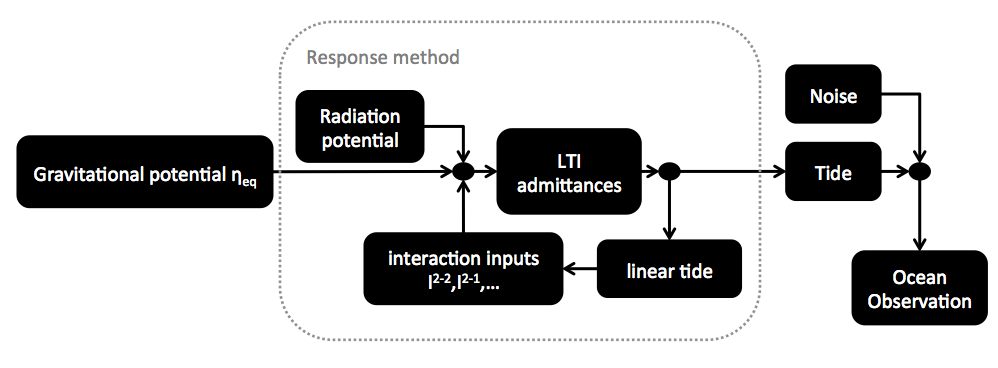
\includegraphics[width=\figwidthBig]{figures/diagrams/response_analysis_flowchart.png}
\caption{Response method tidal schematic.  Nonlinear and non-gravitational inputs are explicitly formed.   Analysis consists of empirically fitting smooth admittance curves.}
\label{fig:response}
\end{center}
\end{figure}

Perhaps even more illustrative of the way in which a response analysis conceptualises tides is the formulation of the `radiational potential'.   This is an additional harmonic forcing series formulated to more explicitly account for the influence of atmospheric tides and other periodic solar effects on ocean observations.	  So-named due to the abstract connection with diurnal solar radiative fluxes, the radiational potential is concept is a little ad hoc in comparison to developments of the \ATGP{}.  The radiational input provided a more satisfactory formulation of observed harmonic ocean signals, S1 and S2, with amplitudes disproportionate to terms in the \ATGP{}.\\
From a sea level forecasting perspective, the response approach could be said to have modernised the formulation and increased the concreteness of the underlying physics, but in doing so hasn't ultimately provide anything more robust and simple for routine use in operational centres.




Fitting a Fourier series vi the convolution formalism to find each smooth admittance is not the only viable implementation of the response concept.  For instance a Green's function formulation is described by Webb\cite{Webb:1974ke} and polynomial models are evaluated by Desai \cite{Desai:1995je}. More influential though is the orthotide approach to fitting Fourier series admittances, discussed below.




% orthotide
A possible weakness of the original convolution formalism in equation \ref{E:lags} relates to the non-orthoganality of the harmonically decomposed $c_{nm}(t)$.  That is, unlike a Fourier series, inner products between component sinusoids comprising the tidal input are not necessarily zero.   Thus the resultant weights $w_{nm}(s)$ are dependant on details of the particular analysis, such as the number of other components included.  The weights cannot be assigned any independent meaning and are not amenable to communication.  In recognising this, Groves and Reynolds \citep {Groves:1975ky} introduced the \underline{orthotide formalism}.\\
Orthotides are orthogalised transformations of the harmonically decomposed tidal input timeseries.

\begin{align}
c_{nm}(t) =  &\sum_{k} H_{nmk} e^{-i(\omega_{nmk} + \beta_{nml})}  \Rightarrow \sum_{l}^L \overline{\zeta}_{nml}(t)     \nonumber \\
             &\mbox{where} \langle \overline{\zeta}_p \overline{\zeta}_q \rangle  = \delta_{pq}  \mbox{over $-\infty < t < \infty$}             \nonumber
\end{align}

A tidal timeseries is then represented as a linear sum of these orthotide functions with `orthoweights'. In essence this is no different to Munk and Cartwrights convolution, but is an improved time-space formulation of equation \label{E:Z}.  The resulting orthoweights have the attractive property of not being dependant on the number of components involved in any particular analysis, and subsequently could be said to share some of the characteristics of conventional tidal constants.
\begin{equation}
\label{E:orthosum}
\eta_{tide}(t) = \sum_{n=2}^3 \sum_{m=0}^n \sum_{l}^L \overline{\zeta}_{nml}(t)
\end{equation}

Regardless of the formulation of time-space convolution, the determination of weights is equivalent to fitting smooth admittance curves - which is the ultimate goal of the response method.  The fitting process is a minimisation problem with degrees of freedom equal to the number of free parameters to be determined.    The length of timeseries and signal to noise ratio are balanced against the assumption of smoothness in $Z$.
\begin{quotation}   
The use of orthotides may provide some benefits to the empirical determination of ocean tide models from a short duration of observations, but is otherwise unnecessary. \dots  polynomial and orthotide, and therefore convolution, approaches to modelling the smooth admittance function provided similar results as long as they are defined by an identical number of parameters.\citep{Desai:2006wo}
\end{quotation}



%-----------------%
\subsection{Tidal admittances in operations}

% LTI
It should be re-iterated that at high level, the harmonic and response models contain the same core concept.   Both model the ocean as an LTI system responding to some type of tidal forcing and both contain assumptions about the smoothness of ocean admittance.  Indeed Le Provost in \citep[chpt6]{Fu:2001ub} groups both the standard harmonic and convolution formalism as instances of the `response' formalism on this basis. \\
By definition these LTI methods are aiming to represent phenomena stationary in tidal frequency-space.  Treatment of non-stationary tidal phenomena forms a scientifically important extension, eg \citep{Colosi:2006va} and \citep{Ray:2011tj}, but presently plays a very secondary role with regard to conventional sea level forecasts.\\
A point of special interest to the explicit resolution of tides within \OGCM{}s is the relatively small but observable sea level surface signatures of nonstationary internal tides.




% harmonics == admitance
Consistent with this equivalence, it is common within the literature to refer to harmonic constants \emph{as} admittances.   A harmonic constant is seen as a sample from the admittance curve at an exact frequency. For instance Smith\cite{Smith:1997ut} provides the simple conversion to sample $Z(\omega_{nmk})$ and scale by the \ATGP{} amplitude $H_{nmk}$.
Furthermore, harmonic constants remain the lingua franca of ocean tide discussions. Regardless of the detail behind any particular method, results are almost universally transformed into conventional amplitude and phase values for intercomparisons.\\
In less specialised language however, harmonic analysis is quite distinct from a response method - especially with regard to whether the outcome is a list of constants or a series of admittance curves.\\




% inference and smooth
Regardless of the method used for analysis, an expectation that admittance curves $Z(\omega)$ should not contain discontinuities or sharp changes (the `credo of smoothness') is commonly evoked to enhance the spectral content upon the \emph{synthesis} of a tidal timeseries.  Following an analysis performed to determine admittances at a relatively small number of frequencies, $Z{\omega}$ is interpolated or extrapolated in frequency-space to infer additional spectral information.   The design of such an inference process can treat frequencies on a case-by-case basis distinguishing between component admittance curves (for instance \citep[pp 268]{Fu:2001ub}).




% operations
There is an apparently wide gap between the practices of centres producing \underline{tide tables} using conventional harmonic analysis and the more varied and advanced methods used within the scientific literature and employed for global models.\\
The relative significance of non-linear effects between the vast open ocean and the coastal zone provides some explanation for this split.  As illustrated in Figure \ref{fig:response}, the manner in which nonlinear feedbacks are incorporated into the response formalism significantly reduces it's elegance in comparison to the purely linear application valid for blue-water tidal analysis.\\
Another factor contributing to this gap is largely cultural.
\begin{quotation}
$\dots$ the improvement in predictable variance is numerically small compared with the natural noise in sea level.   Because of this, and the fact that the Response Method is harder for a routine operator to grasp, it has never been adopted for ordinary tide-table production. It remains essentially a research tool for specialists. \citep[pp 198]{Cartwright:2000tt} 
\end{quotation}
Expanding Cartwright's explanation, the importance of robustness and intuitive error checking to routine operations should also be emphasised.  Short tables of constants are indeed physically intuitive and facilitate simple checking.   And the presentation of spatial atlases for amplitude and phase are standard.





%-----------------%
\subsection{Distinguishing forecasts and filtering}

Sea level forecasting is not the only reason for employing tidal methods in operational centres.\\
Tidal methods are employed for two broadly distinct purposes: forecasting and filtering.  And beyond the operational context even more varied tidal methods are employed for data analysis and specialised studies.\\

The distinct motivations behind producing a forecast and filtering a signal can lead to significant differences in what is defined as the tidal component of observed sea level.   Subsequently, apparently inconsistent tidal timeseries can be in simultaneous use within an operational centre.



Filtering to remove tides from an ocean signal is commonly referred to as `de-tiding'.  Filtering is a means to distinguish signal and noise.  Application of a de-tiding process categorises tidal variations as noise so as to make use of the remnant signal.   In that respect de-tiding is nominally the inverse problem to tidal analysis.   Following the discussions in Section \ref{SS:semantics}, important details regarding what should be defined as tidal then naturally depend on the context of an application.\\
Operational oceanography in the form of \BL{} relies on de-tided altimetry observations as an important assimilation constraint.   The de-tiding process has been designed to render the observations compatible with the physics of the model, with a focus on meso-scale baroclinic variability. The current configuration of \BL{} does not assimilate tide gauge data, though in principle these insitu observations could be rendered consistent via appropriate de-tiding, for example \cite{Matsumoto:2000tg}.\\


\begin{figure}[h]
\begin{center}
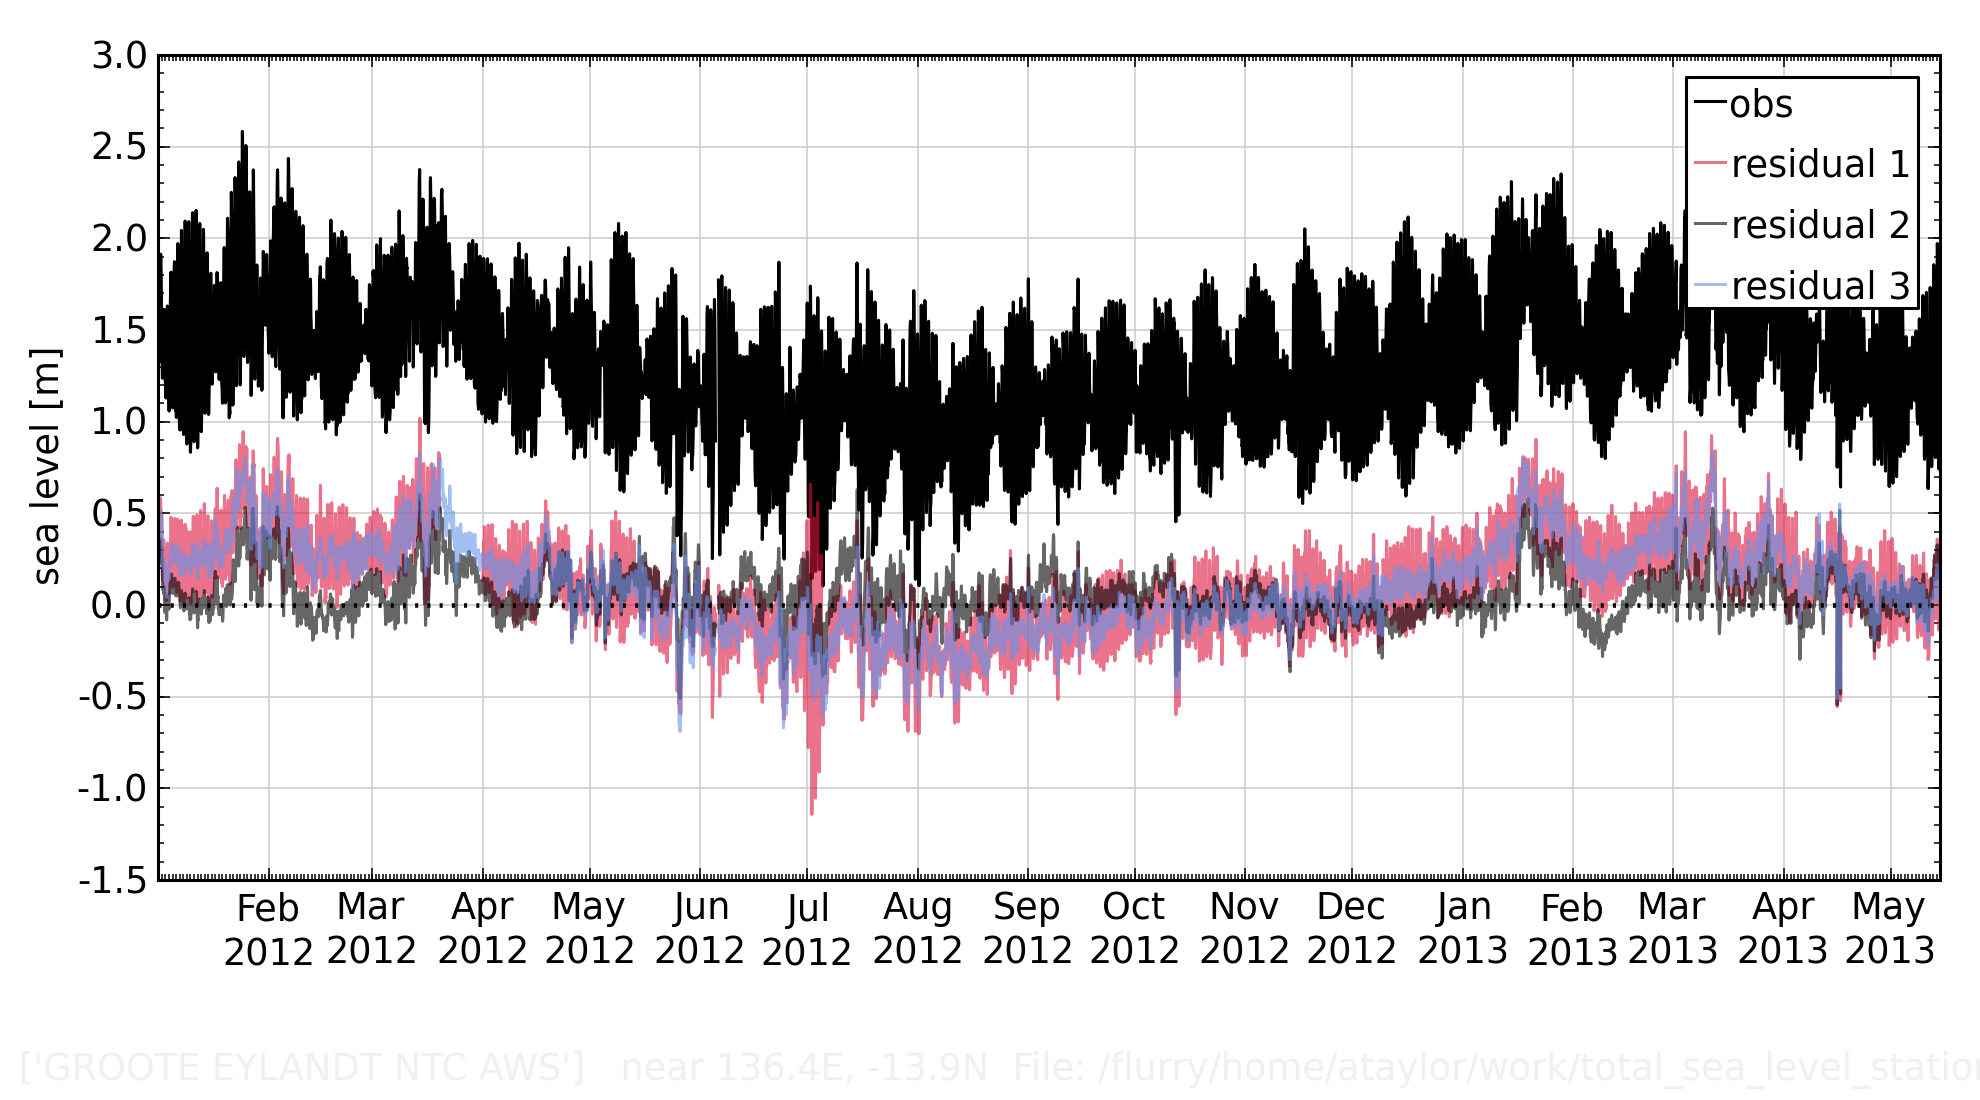
\includegraphics[width=\figwidthFull]{figures/plots/diag_plot_014406_detide_compare_20120101.png}
\caption{Illustration of de-tiding observations by subtraction of tide predictions.  Different `residuals' result from alternative tide predictions: [1] regional gridded tide solution, [2] harmonic prediction and [3] harmonic prediction with significant non-gravitional harmonics removed. }
\end{center}
\end{figure}


Altimetry observations are de-tided via subtraction of a tidal signal synthesised from a global model.  There is no unique manner in which to specify the correction, with many options and `flavours' available from standard sources such as RADS \citep[table 3.2]{Scharroo:2011vd}.  The details of how the tidal correction is constructed can have implications for interpretation of the final ocean forecast.   The treatment of long-period tides \citep{Egbert:2003jd} and nongravitational tides \citep{Arbic:2005gv} are highlighted as special points of interest with regard to operational sea level forecasts.\\




In contrast to the situation with filtering, dynamical cause and effect are only relevant to stand-alone tidal forecast products insofar as they impact predictability.  From a users perspective, tide tables simply forecast sea level and ideally account for as much of the observed signal as possible.   By that measure it is proper that the tide tables include all of the reliably periodic signal regardless of cause.   
Thus the treatment of long-period harmonics Sa and Ssa is `philosophical question' \citep{Parker:2007wq} insofar as any reliably periodic signal at these relatively low frequencies can be determined from the observational record.  It is then not surprising that even amongst Australian tide authorities treatment of long-period signals differs enough to warrant special review attention{MHL:2013perscomm}.


TBC ref to chapter.

% wavelets etc
For completeness it should be mentioned that other analysis techniques exist in the literature that are less directly relevant to the provision of sea level forecasts.\\
For instance, specifically tidal applications of wavelet analysis have been described as tools to provide insight into non-stationary tidal processes \citep{Flinchem:2000kp}.



%-----------------%
\subsection{Distinguishing insitu and spatial tide models}

Satellite altimetry motivated the extension of the empirical analysis methods discussed above to the production of regional and global atlases of ocean tides.  Indeed, tidal analysis formed an important driver and design constraint on the development of satellite altimetry missions.\\
Global tide models are commonly employed as intermediate products for other calculations well beyond the purposes of sea level forecasting per se.  For instance in the quantification of gravity effects, orbit determination, earth rotation and even the definition of coordinate systems \citep{Anonymous:2004tm}.\\



Meaningful tidal atlases existed prior to altimetry, most significantly that due to Schwiderski \citep{Schwiderski:1983ke}, but these necessarily suffered from a lack of validation and constraint in the deep ocean.\\
The basic premise of a tidal atlas is to present maps of tidal admittance at discrete frequencies, typically as separate amplitude and phase diagrams.   In line with the discussion in Section \ref{S:LTI}, the deep ocean is conceived as a LTI system that is by definition stationary.  Each component wave can also be called a partial tide.\\
It is conventional to present atlas tidal predictions as separate maps of amplitude and phase for a single frequency.  These are also called `co-tidal' and `co-range' plots.  This visualisation fits well with the concept of the tidal ocean as a linear sum of standing waves.   The long spatial scale of these component waves and the existence of spatial nodes places special importance upon \emph{amphidromes} or \emph{amphidromic points} - nomenclature introduced by Harris in the late 19th century \cite[pp 119]{Cartwright:2000tt}.  Existence and placement of amphidromic points is an important visual metric employed to assess tidal model results \citep{foreman:2012perscomm}.  Figure \ref{fig:atlas} shows a the typical tidal atlas result with amphidromic systems apparent as radial patterns in the co-phase diagram.\\
Modern tidal atlases are in close agreement with regard to broad patterns, but characteristically differ at the shallow water margins; the very location of most direct interest to sea level forecasts.  Figure \ref{fig:tpx_cross} illustrates the fact that modern global tide models typically agree within about 0.02m in the deep ocean, but can differ substantially in coastal and shelf regions.  


\begin{figure}[h]
\begin{center}
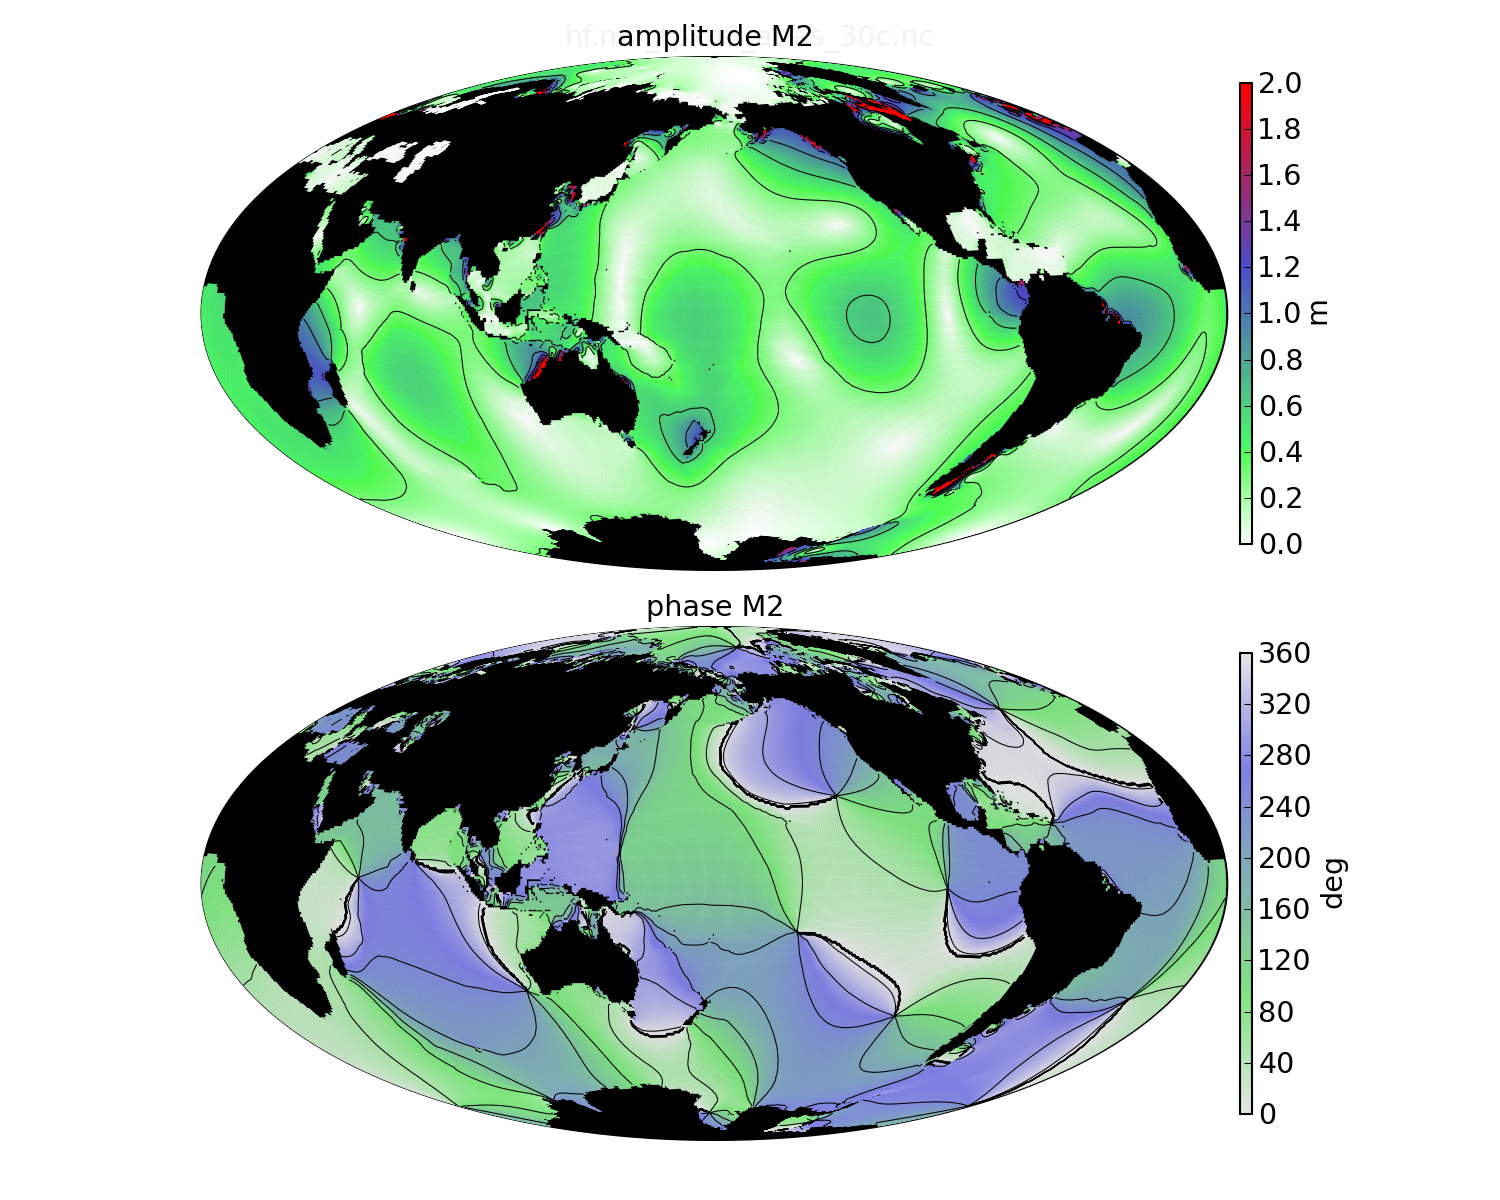
\includegraphics[width=130mm]{figures/maps/global_m2_tpx08.png}
\caption{Example tidal altas showing cophase and corange diagrams for a single tidal component M2.  Data source TPX08 \cite{Egbert:2002ug}  }
\label{fig:atlas}
\end{center}
\end{figure}


\begin{figure}[h]
\begin{center}
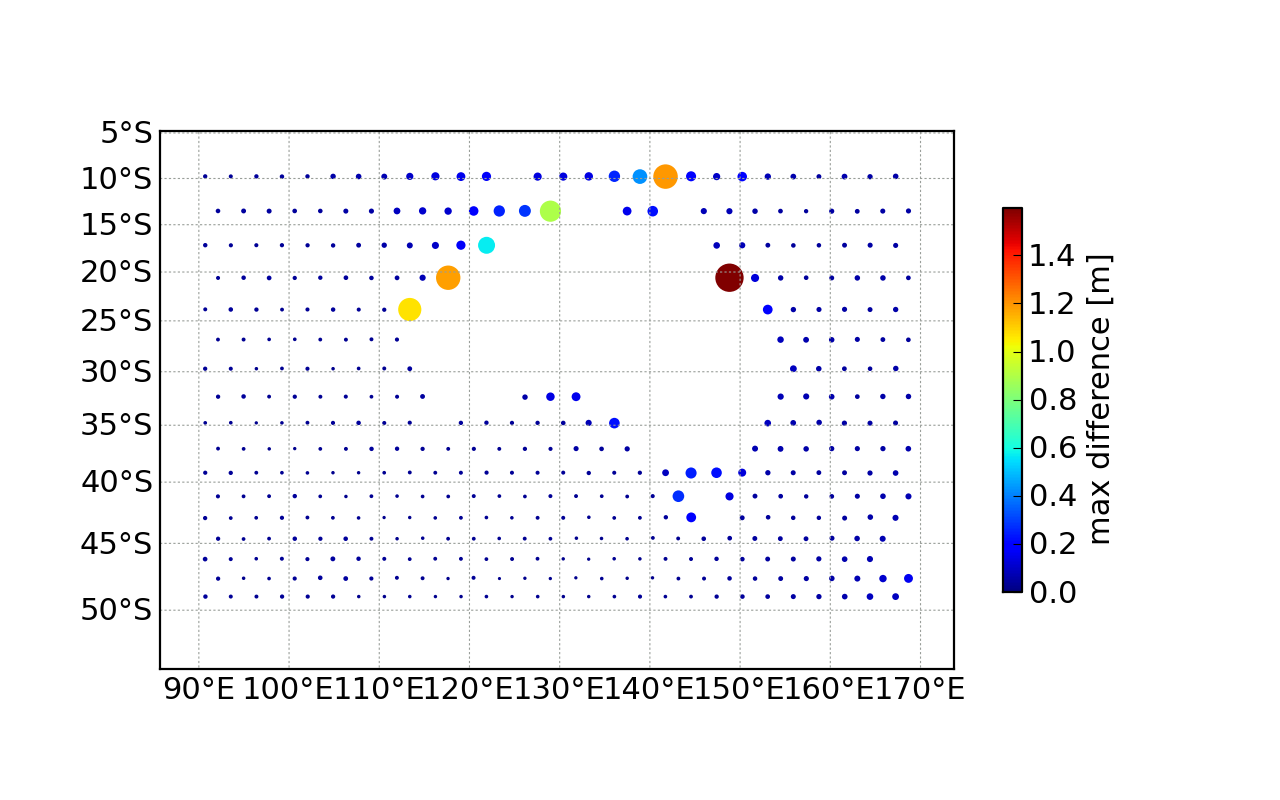
\includegraphics[width=110mm]{figures/maps/map_tide_differences_tpx_xovers.png}
\caption{Maximum difference between tidal timeseries for 2012 at topex cross-overs near Australia.  The different solutions agree very closely in deep water, whilst the significance of shallow water effects are apparent.  Models included: CSR04\citep{Eanes:1996tr}, FES04\citep{Lyard:2006ir}, DTU10\citep{IMPROVEMENTOFGLOBA:2010tu}, GOT47, GOT48\citep{Schrama:1994vr}\citep{Ray:1999vm} }
\label{fig:tpx_cross}
\end{center}
\end{figure}


The LTI concept embodied in tidal atlases is well suited to representing deep water tides.   Amplitudes of each partial tide are no larger than about 0.02 cm for the majority of the global ocean, compared to depths of around 4km.
Given the underlying LTI framework, the tidal literature has naturally focused on stationary frequency-space metrics.  Intercomparison of mode1s and assessment against observations is almost always performed at a small set of dominant tidal frequencies - commonly only M2, K1, O1 and S2.\\
Tidal atlases are in essence no different from one-dimensional tide predictions.   Preceding discussions regarding the varied formalisms [Section \ref{S:formalisms}] apply equally to regional atlases as to insitu timeseries.  Similarly to insitu tidal products, special attention is warranted regarding the treatment of signals associated with non-gravitational effects and the possible differences between a forecast model and an correction/filter.\\



Whilst some authors have presented the existence of repeat-orbit altimetry observations as effectively being `thousands of tide gauges', reduction of these observations via tidal analysis requires many special considerations.  For instance, infrequent but regular observation of any one surface coordinate places special importance on aliasing effects.\\



Despite the general equivalence, a point of practical difference is the treatment of the non-linear effects significant in shallow water.\\
In contrast to the apparent convergence of surface tide models in the open ocean, shelf and coastal regions are problematic.   In shallow waters wavelengths shorten and nonlinear interactions between partial tides can become very prominent.  \\
A strength of conventional 1-dimension analyses of coastal tide gauges has been the incorporation of shallow water compound tides.  It is not atypical in Australian locations to include dozens of nonlinear frequencies in a harmonic analyses.   Nonlinear signals observed at a tide gauge are often due to complex very localised dynamics, and the spatial projection beyond the observation point is non-trivial.  Understandably, global tidal atlases have generally focussed attention on the linear deep water signal and have poorly represented or ignored coastal nonlinearties.  The nonlinear M4 signal (associated with self-interaction of M2 waves) is perhaps the only such partial tide to be included in many modern atlases and is observable with altimetry \cite{Ray:2010jm}.\\



As a forecast product, tidal atlases have nothing like the broad economic integration of conventional coastal tide tables.  The Australian Bureau of Meteorology does not promulgate official tide predictions away from insitu observation locations. \\
For the contemporary operation setting, tidal atlases are primarily relevant as an intermediate product to enable satellite observations.



Coordinated development of improved tidal atlases with specific performance requirements formed a significant component of altimetry missions in the 1990s.
\begin{quotation}
This international effort quickly split into two main approaches: the so-called empirical approach based on the direct analysis of the altimetry sea level time series \dots{}, and a modelling approach based on hydrodynamic and assimilation models. Later on, the interaction between the two approaches (i.e. data assimilation based on altimetry analysis on one hand, and hydrodynamic/assimilation modelling on the other hand) was a key factor for the overall success in improving tidal prediction accuracy and reaching the T/P requirements \cite[pp394]{Lefevre:2011dg}.
\end{quotation}




%%-----------------%
%\subsection{Global tide solutions and data assimilation}

TBC!! 
No global tidal atlas can be purely empirical - the spatial and temporal coverage of observations is too sparse.\\
Schwiderski's pre-altimetry solutions relied heavily on global compilations of harmonic constants for mainly coastal tide gauges, from which spatial maps were created via a `hydrodynamic interpolation' method that would in hindsight be considered an application of data assimilation \cite[pp822]{Egbert:1994wz}.\\
Now with around 20 years of altimetry data, all the highly evolved global tidal models or \emph{tidal solutions} in use all employ data assimilation in some manner.  That is, they make some combined use of dynamic models and observational data.  This includes a reliance on supporting geophysical models and corrections implied by the use of altimetry observations.\\



The dynamics relevant to tidal sea level are conventional written as the Laplace Tidal Equations (LTE) - for instance \cite[9.8]{gill1982atmosphere} and \cite{Hendershott:1981ub}.   
Via a series of assumptions, the LTE are a set of depth integrated shallow water equations in a rotating thin shell.  Advection is neglected altogether.\\
The LTE evolve a simple 3 dimensional ocean state consisting of horizontal mass transport and sea level perturbation. In time domain, the LTE can be written following the notation and discussion of \cite[pp185]{Egbert:2002ug}:

% LTE in time-domain
\begin{align}
\label{E:LTE_momtm}
\frac{\delta \mathbf{U} }{ \delta t} + f\vec{k} \times \mathbf{U} + gH\nabla \eta  + \mathbf{F} &= \mathbf{f_0} + gH \nabla \eta_{SAL} \\
\label{E:LTE_cont}
\frac{\delta \mathbf{\eta} }{\delta t} &= -\nabla.\mathbf{U} 
\end{align}

Where $\mathbf{U}$ is the depth integrated horizontal transport, $\eta$ is the sea level signal, $H \gg \eta$ is mean water column depth, $f=2\Omega\sin\theta$ is the Coriolis parameter and $g$ vertical gravitation.\\
The forcing terms on the right hand side of the momentum equation \label{E:LTE_momtm} require explanation.  
$\mathbf{f_0}$ denotes the astronomical body forcing taking into account earth tide effects, $\mathbf{f_0} = gH\nabla\eta_{eq}$ following Equation \ref{eq:VT}.  
An approximation for SAL is here written as a separate forcing term to reflect the suitability of using values pre-computed from existing global tide models.   
Alternatively $\eta_{SAL}$ can be put on the left hand side of the equation as a scaled version of $\eta$ - as is the case in \MOM{}.   
This scalar approximation is relatively inaccurate as discussed in section \ref{sec:basic_potential}.\\
The frictional dissipation term $F$ is a particular source of complexity, especially with regard to parameterisation and linearisation.\\

Compared to the dynamics represented within an \OGCM{}, these tidal hydrodynamics simulate a more `aggregated' psuedofluid in that the processes contained within parameterisations are have a higher degree of complexity - as per the schematic in Figure \ref{fig:models} \\
\begin{quotation}
Forward global tide models are an ideal testing ground for the hydrodynamical cores of numerical ocean general circulation models, and for ideas about drag and dissipation. In contrast to data-constrained models, forward models cannot achieve accurate tidal elevations unless substantial parameterised drag is included in the abyss. Forward models thus point clearly to drag in the open ocean as a central control on tidal flow.\citep{Arbic:2004wz}
\end{quotation} 


Linearisation is important in the tidal context to facilitate transformation of the LTE into the frequency domain.   Given the tidal LTI framework, the ultimate solution of a tidal model is the evaluation of static admittances or constants.   One approach towards this end would be to integrate the LTE in the time-domain and subsequently reduce the output to a series of harmonic constants via conventional analysis.   The celerity of barotropic waves in the deep ocean is relatively fast and thus requires short time-steps.   Assuming linearity and the existence of a convergent solution in frequency-space, the LTE can be solved directly in spectral form with greater computational efficiency.   The efficiencies are especially important upon the application of data-assimilation methods that involve both a backward and forward iteration of the dynamics \cite[pp184]{Egbert:2002ug}.


Again following the notation of \cite[pp186]{Egbert:2002ug}, the LTE at a single tidal frequency $\omega$ can be written:

% LTE in freq-domain
\begin{align}
\label{E:LTE_momtm_w}
\mathbf{\Omega} \mathbf{U} + gH\nabla \eta &= f_u \\
\label{E:LTE_cont_w}
\nabla.\mathbf{U} + i\omega\eta &= f_\eta\\
\mbox{where   } \Omega             &=
\left[ \begin{array}{cc} 
      i\omega + \kappa & f \\ 
       -f              & i\omega + \kappa  
                        \end{array} \right]   \nonumber
\end{align}

Where $\kappa$ is a linearised approximation for the dissipative stress.   Frequency-space forcing terms $f_u, f_\eta$ are written in both equations for generality with regard to data assimilation (inversion).  This frequency-space approach is common to other data assimilative tidal models such as FES \cite[pp395]{Lyard:2006ir}.\\
Nonlinear terms can be incorporated but complicate the formulation of any inversion.



Whilst numerically solving the LTE is quite tractable and comparatively simple, significant uncertainties prevent a direct `free' or `forward' model from producing accurate forecasts.  Hence the importance of data assimilation or generalised inversion methods.  Solving the LTE is complicated by spare observations and ``$\dots$ the need for accurate open boundary conditions and bottom topography, the need for approximate parameterisations of dissipation in the tidal equations, solid earth effects, and the effects of ocean stratification on the barotropic tides, which may be difficult to account for without full 3D modelling of baroclinic tidal currents''\citep[183]{Egbert:2002ug}.\\
A comparative description of data assimilation methods in the context of tide models is laid out by Egbert and Bennet \cite{Egbert:1996vr}.\\   



Summaries that categorise the many global tide models on the basis of design choices, parameterisations and data assimilation methods are given in \cite{Ardalan:2008gs} and \cite{Matsumoto:2000tg}. \\

%   ??  Application of the LTE is not restricted to the barotropic surface tide.   The formulation can be extended to represent stationary internal tidal modes via use of equivalent-depths .\\
% Energy cascades.??\\

The barotropic hydrodynamics used in global tide models has proven to be an appropriate level of aggregation when the aim is to map tidal patterns of surface elevation.  The LTE provide a tractable means of doing so given the incomplete spatial and temporal coverage of observations.\\
But consideration of tidal dynamics naturally raises the topic of \emph{internal tides} and the separability of stationary barotropic tides from other ocean dynamics.\\
\begin{quotation}
Barotropic tides generate internal tides, and internal tides in turn feed back onto the barotropic tides. Inferences from altimetry-constrained barotropic tide models show that about one-third of global tidal energy dissipation occurs in regions of rough topography, where internal tides are generated \dots{}. Internal tide generation thus acts as a damping mechanism for the barotropic tides.\citep[pp22]{Arbic:hy}
\end{quotation}
Depth integrated barotropic LTE relegate the effect of internal mechanisms on surface elevation to parameterisations.  Dissipative stress $F$ in \label{E:LTE_momtm} stands for all losses of energy from the barotropic pseudofluid.  Given the reality of ocean stratification, these losses notably include conversion form the barotropic to higher baroclinic modes \cite[pp121] {gill1982atmosphere}. \\



For the present topic of sea level forecasting, internal modes are ostensibly of interest insofar as they impact the prediction of surface elevation.  Internal waves at tidal frequencies do have an observable surface signature albeit relatively small \cite{Ray:2011tj}.\\
More importantly for forecasting is the effect of the internal ocean state on the prediction of barotropic surface elevation.  A-periodic variation of the internal density structure of the ocean is of particular relevance as   conventional tidal analysis relies upon periodicity for predictability.     The tidal view of the ocean as a LTI system driven by the \ATGP{} is very useful, but with the caveat that ``the ocean is a physically complex and noisy filter.  In consequence, tidal harmonics are not strictly constant \citep[197]{Ray:2010jm}''.\\



Whilst stratification and internal mechanisms are very coarsely parameterised in dedicated tidal models, the internal structure of the ocean is a primary focus of \OGCM{}s.   The following section addresses the intersection of \OGCM{}s and tidal forcing with regard to sea level forecasts.


%-----------------%
\subsection{No singular ocean tide requirement in operations}

TBC .... 
whereas tidal manuals exist such as \citep{PCTMSL-sp9}, \citep{IOC:2005tj}, \citep{Level:2011wu}and \citep{Parker:2007wq} the operational details of practices are not generally published. 



A range of auxillary and derived from conventional tidal methods
- reference planes like HAT
- 



This lack of clarity motivates proposal in Chapter \ref{chp:tideFlavours}



detiding filter for non-tidal models taken up in the next section ....